\documentclass[a4paper,12pt]{article}

\usepackage[utf8x]{inputenc}
\usepackage[english,romanian,hungarian]{babel}
\usepackage[margin=1in]{geometry}

\usepackage{indentfirst}
\usepackage{fancyhdr}
\pagestyle{fancy}

\usepackage[table,xcdraw,dvipsnames]{xcolor}
\definecolor{whitesmoke}{rgb}{0.96,0.96,0.96}
\definecolor{lightblue}{rgb}{0.22,0.45,0.70}
\definecolor{darkred}{rgb}{0.9,0.0,0.0}

\usepackage[unicode,backref=false,pagebackref=true]{hyperref}
\hypersetup{colorlinks=true,urlcolor=lightblue,citecolor=green!75!black,linkcolor=orange!98!black,pdfborder={0 0 0}}
\usepackage[all]{hypcap}
\usepackage{multirow}

\usepackage{graphicx}
\usepackage{wrapfig}

\usepackage{booktabs}
\usepackage{multicol}
\usepackage{amsmath}

\usepackage{tikz}
\usetikzlibrary{arrows}
\tikzstyle{es} = [-triangle 60]

\usepackage{enumitem}
\setlist[itemize]{itemsep=0pt}
\setlist[enumerate]{itemsep=0pt}

\setlength{\parindent}{2em}
\setlength{\parskip}{0.25em}

\renewcommand{\arraystretch}{2}

\usepackage[T1]{fontenc}
\usepackage{lmodern}
\usepackage{fontawesome}

\newcommand{\urlprefix}{Retrieved from \urlstyle{rm}}

\newcommand{\refspace}{\vspace{-2mm}}
\newcommand{\redarrow}{\textcolor{darkred}{$\mathbf{\to}$}}
\makeatletter
\def\BR@@bibitem#1#2\par{
	\let\backrefprint\BR@backrefprint
	\def\@linkcolor{black}
	\BRorg@bibitem{#1}#2\redarrow \thinspace \BR@backref{#1}
}
\makeatother

\usepackage{titlesec}
\titleclass{\subsubsubsection}{straight}[\subsection]

\newcounter{subsubsubsection}[subsubsection]
\renewcommand\thesubsubsubsection{\thesubsubsection.\arabic{subsubsubsection}}
\titleformat{\subsubsubsection}
  {\normalfont\normalsize\bfseries}{\thesubsubsubsection}{1em}{}
\titlespacing*{\subsubsubsection}
{0pt}{3.25ex plus 1ex minus .2ex}{1.5ex plus .2ex}

\makeatletter
\def\toclevel@subsubsubsection{4}
\def\l@subsubsubsection{\@dottedtocline{4}{7em}{4em}}

\renewcommand\paragraph{\@startsection{paragraph}{6}{\parindent}%
  {3.25ex \@plus1ex \@minus .2ex}%
  {-1em}%
  {\normalfont\normalsize\bfseries}}
\makeatother

\setcounter{secnumdepth}{4}
\setcounter{tocdepth}{4}

\makeatletter
\newcommand\hungariantableofcontents{%
  \selectlanguage{hungarian}%
  \section*{\contentsname
    \@mkboth{\MakeUppercase\contentsname}{\MakeUppercase\contentsname}}%
  \@starttoc{toc.hu}%
  \selectlanguage{english}%
 }
\makeatother

\newcommand\sectionhu[1]{\addcontentsline{toc.hu}{section} {\protect\numberline{\thesection} #1}}
\newcommand\subsectionhu[1]{\addcontentsline{toc.hu}{subsection} {\protect\numberline{\thesubsection} #1}}
\newcommand\subsubsectionhu[1]{\addcontentsline{toc.hu}{subsubsection} {\protect\numberline{\thesubsubsection} #1}}
\newcommand\subsubsubsectionhu[1]{\addcontentsline{toc.hu}{subsubsubsection} {\protect\numberline{\thesubsubsubsection} #1}}

\makeatletter
\newcommand\romaniantableofcontents{%
  \selectlanguage{romanian}%
  \section*{\contentsname
    \@mkboth{\MakeUppercase\contentsname}{\MakeUppercase\contentsname}}%
  \@starttoc{toc.ro}%
  \selectlanguage{english}%
 }
\makeatother

\newcommand\sectionro[1]{\addcontentsline{toc.ro}{section} {\protect\numberline{\thesection} #1}}
\newcommand\subsectionro[1]{\addcontentsline{toc.ro}{subsection} {\protect\numberline{\thesubsection} #1}}
\newcommand\subsubsectionro[1]{\addcontentsline{toc.ro}{subsubsection} {\protect\numberline{\thesubsubsection} #1}}
\newcommand\subsubsubsectionro[1]{\addcontentsline{toc.ro}{subsubsubsection} {\protect\numberline{\thesubsubsubsection} #1}}

\usepackage{minted}
\renewcommand{\theFancyVerbLine}{\rmfamily\scriptsize\arabic{FancyVerbLine}}
\setminted{linenos,autogobble,breaklines,fontsize=\footnotesize,tabsize=4,numbersep=7pt,bgcolor=whitesmoke}
\AtBeginEnvironment{minted}{\renewcommand{\fcolorbox}[4][]{#4}}

\author{Roland Bogosi}
\title{Black-Box Penetration Testing and Vulnerability Management Platform}

\PrerenderUnicode{áéúóőűíăâîșț}

\begin{document}

%
%	Hungarian Section (Summarized Version)
%

\pagestyle{empty}
\selectlanguage{hungarian}

	\begin{center}
		{\Large Sapientia Erdélyi Magyar Tudományegyetem}\\\vspace{0.05in}
		{\Large Műszaki és Humántudományok Kar, Marosvásárhely}\\\vspace{0.07in}
		{\Large Számítástechnika}\\
		
		\vspace{2.5in}
		
		{\huge Behatolástesztelő és Sebezhetőségfelderítő}\\\vspace{0.1in}
		{\huge Rendszer}
		
		\vspace{0.5in}
		
		{\LARGE Szakdolgozat -- Kivonat}
		
	\end{center}
	
	\vspace{2.0in}
	
	\begin{multicols}{2}
		\begin{flushleft}
			{\Large Vezető tanár:}\\\vspace{0.1in}
			{\LARGE {Dr. Vajda Tamás}}
		\end{flushleft}
		\columnbreak
		\begin{flushright}
			{\Large Diák:}\\\vspace{0.1in}
			{\LARGE {Bogosi Roland}}
		\end{flushright}
	\end{multicols}
	
	\vspace{1.5in}
		
	\begin{center}
		{\LARGE 2016}
	\end{center}

\newpage
\section*{Tartalomjegyzék}

	\begingroup
	\renewcommand{\section}[2]{}
	\hypersetup{linkcolor=lightblue}
	\setlength{\parskip}{0em}
	\hungariantableofcontents
	\endgroup

%
%	Romanian Section (Summarized Version)
%

\newpage
\pagestyle{empty}
\selectlanguage{romanian}

	\begin{center}
		{\Large Universitatea Sapientia, Târgu-Mureș}\\\vspace{0.05in}
		{\Large Facultatea de Științe Tehnice și Umaniste}\\\vspace{0.07in}
		{\Large Calculatoare}\\
		
		\vspace{2.5in}
		
		{\huge Sistem pentru Teste de Penetrare și}\\\vspace{0.1in}
		{\huge Descoperirea Vulnerabilităților}
		
		\vspace{0.5in}
		
		{\LARGE Teză de Licență -- Extras}
		
	\end{center}
	
	\vspace{2.0in}
	
	\begin{multicols}{2}
		\begin{flushleft}
			{\Large Îndrumător Științific:}\\\vspace{0.1in}
			{\LARGE {Dr. Vajda Tamás}}
		\end{flushleft}
		\columnbreak
		\begin{flushright}
			{\Large Absolvent:}\\\vspace{0.1in}
			{\LARGE {Bogosi Roland}}
		\end{flushright}
	\end{multicols}
	
	\vspace{1.5in}
		
	\begin{center}
		{\LARGE 2016}
	\end{center}

\newpage
\section*{Cuprins}

	\begingroup
	\renewcommand{\section}[2]{}
	\hypersetup{linkcolor=lightblue}
	\setlength{\parskip}{0em}
	\romaniantableofcontents
	\endgroup

%
%	English Section (Full Version)
%

\newpage
\pagestyle{empty}
\selectlanguage{english}

	\begin{center}
		{\Large Sapientia University, Târgu-Mureș}\\\vspace{0.05in}
		{\Large Faculty of Technical and Human Sciences}\\\vspace{0.07in}
		{\Large Computer Engineering}\\
		
		\vspace{2.5in}
		
		{\huge Black-Box Penetration Testing and}\\\vspace{0.1in}
		{\huge Vulnerability Management Platform}
		
		\vspace{0.5in}
		
		{\LARGE Bachelor's Thesis}
		
	\end{center}
	
	\vspace{2.0in}
	
	\begin{multicols}{2}
		\begin{flushleft}
			{\Large Supervisor:}\\\vspace{0.05in}
			{\LARGE {Dr. Tamás Vajda}}
		\end{flushleft}
		\columnbreak
		\begin{flushright}
			{\Large Student:}\\\vspace{0.1in}
			{\LARGE {Roland Bogosi}}
		\end{flushright}
	\end{multicols}
	
	\vspace{1.5in}
		
	\begin{center}
		{\LARGE 2016}
	\end{center}

\newpage
\pagestyle{empty}
\section*{Table of Contents}
\selectlanguage{english}

	\begingroup
	\renewcommand{\section}[2]{}
	\hypersetup{linkcolor=lightblue}
	\setlength{\parskip}{0em}
	\tableofcontents
	\endgroup

	\begingroup
	\hypersetup{linkcolor=lightblue}
	\listoffigures
	\listoftables
	\listoflistings
	\endgroup

\newpage
\pagestyle{fancy}
\selectlanguage{english}
\section{Introduction}
\sectionhu{Bevezető} \sectionro{Introducere}

	As the world is embracing digital technologies more and more, a lot of our services are keeping up with this trend, and have started being digitally available for the purposes of easier and faster accessibility. Digital data can be processed much faster and reliably than its analogue equivalents, which benefits the service providers by keeping the costs of providing their services low. Customers are also saved the headache of experiencing routine unpleasantries which are now alleviated by digital services, such as queuing up in order to pay the bills for various services one has subscribed to.
	
	Service providers, however, are not the only consumers of the benefits handed to us by the Internet. Advancements made in the past decade in the fields of software, hardware and network connectivity, have led to an exponential growth in the number of devices connected to the Internet. Due to the boom of \textit{IoT}, (``\textit{Internet of Things}'') \textit{Cisco} predicts there will be 25 billion devices connected to the Internet by 2015, which number is expected to increase to 50 billion by 2020.\cite{devans11} The pool of unallocated IPv4 addresses was completely depleted when \textit{LACNIC} has allocated their last block on the 10th of June, 2014.\cite{ghouston11} This event symbolically signifies, that the Internet has become way too big for what it was initially envisioned in the 1960's.
	
	Our increasing reliance on digital services and data are not without its drawbacks, however. With more and more sensitive information and transactions being done over the Internet, one must question the security of it all. As one idiom states, ``\textit{a chain is as strong as its weakest link},'' and in the context of Internet-enabled applications, there are a lot of these aforementioned figurative ``\textit{links}.'' Starting from the possibility of there being an attack vector on any layer of the \textit{OSI} between the two communicating devices, down to the vulnerabilities which are specific to the application being executed over the network.
	
\subsection{Security Awareness of IT Professionals}
\subsectionhu{Biztonsági Tudatosság az IT Szakértőkben} \subsectionro{Conștientizarea Importanței Securității -- Profesioniștilor IT}
	
	As one study done by \textit{BSIMM-V} (\textit{Building Security in Maturity Model}) which included 51 top-tier firms (mostly fortune 500) has concluded\cite{gmcgraw12}, a large percentage of product managers, software developers and system administrators have never received security awareness training nor been instructed to lay an emphasis on security, and as a result they do not prioritize it. One of the reasons why one might \textit{not} consider security awareness to be a priority is due to bogusly thinking that security aware application development and deployment is too costly. A study done by the \textit{Aberdeen Group} has shown that companies who invest in security end up with up-to a four-fold \textit{ROI} (``\textit{Return on Investments}'').\cite{aberdeen11}
	
	Companies have a long history of showing ignorance instead of security awareness. They are continuously claiming that they are untouchable, however, this is simply not true and these companies have been proven wrong time and time again. One recent example would be \textit{General Motor}'s take on their Internet-connected cars, where their spokesperson claimed that their cars are not ``hackable'' due to the fact that their entertainment system is separate from the rest of the control systems. A vulnerability was found by two security researchers\cite{cmiller15} which allowed them to inject control messages into the car's CAN bus, effectively allowing them to take control over the car via either Wi-Fi or GSM.
	
	Software developers who would like an introduction to security-aware development can look up many of the freely available resources, however, this is not a perfect substitute for the proper training and the appropriate mindset. In some of the times, a vulnerability that was introduced by a developer might not even be their own fault, as more factors come into play in such cases. A developer might be familiar with the quirks and security issues of a specific language/environment/stack, but then be required by circumstance to move out of their comfort zone and either implement a given task in a non-standard way, or in a language they are not familiar enough with.
	
	One such case would be a developer of a managed language (for example, C\#) be required to interface with a non-managed language (for example, a library written in C) in which case the developer is now expected to do memory management in a language that does not promote its language management tools for it is a managed language. If said library is more complex, there are very high chances, that the developer will overlook some aspects (or not be aware they must be considered in the first place) and undesirable consequences may start happening, such as memory leaks and buffer over/underflows. In such case, it is recommended that a seasoned developer write a wrapper for the specific library in \textit{C++/CLI} (successor of \textit{Managed-C++}), a language designed by Microsoft for the intent purpose\cite{hstutter06} of bridging the managed and unmanaged worlds.
	
	There are other special circumstances under this argument, for example situations in which the developer of the application might be security-aware, or a proper penetration testing/code review was done, but the proposed security fixes might impact performance, ease of use, or even cause minor to major discomfort for the users. In such cases, risk analysis will be done, and some of these proposed solutions will be rejected as being unjustifiably too obtrusive. It is not the \textit{right} course of action in such situations, but risk analysis[\ref{ssec:vulnriskanal}] is a pretty standard tool for decision makers.
	
	Another special case would be IoT device ideas that have been funded through the use of crowdfunding platforms. These platforms, such as Kickstarter or IndieGoGo, are the hotbed of young entrepreneurial spirits with fresh ideas wanting to procure enough money in order to have a chance at executing them. Early prototypes of these projects are generally crafted using existing prototyping boards, such as Arduinos and Raspberry PIs. Later, when the proof of concept has proven to be viable and the first batch is moved to manufacturing, a similar architecture is built so as to allow reuse of existing code. This generally means that experimental code written in an environment in which the developer might not be comfortable enough in, is now being shipped as production code. This practice has spawned in the past lots of devices that are vulnerable and might present a huge security risk.\cite{mstan14}
	
\subsection{Security Awareness of Home Users}
\subsectionhu{Biztonsági Tudatosság az Otthoni Felhasználókban} \subsectionro{Conștientizarea Importanței Securității -- Utilizatorilor Casnici}
	
	As Internet-connected devices are becoming more and more affordable and easier to use, home users have started adopting more and more of these devices. Unfortunately, home users never receive any sort of formal security awareness training, and as such are very easily persuaded to fall for any type of attack which could have been easily prevented had they received a minimal amount of training. Even though, best-practices are usually laid out in the manual of the software being used, users tend to apply ignorance\cite{jnielsen12} even in cases when important notices and warnings are being displayed on the interface of the software and automatically click the ``OK''/``Next'' buttons, whatever gets them to what they wanted to be doing in the first place.
	
	A study done by the \textit{Colorado State University} has had some interesting\cite{ahowe12} results. When testing a group of people self-identified as having \textit{high} to \textit{very high} security awareness, 68\% of them ignored certificate errors on an HTTPS connection, and tried to determine the legitimacy of the said site based only on its content.
	
	A similar survey done in the U.K. has determined\cite{sfurnell07} that 93\% of the surveyed users has had some sort of anti-virus software installed, but only 50\% have installed it for themselves, and while this last point would not be an issue in and of itself, only 37\% of the respondents were applying security patches to their operating system on an at least weekly basis.
	
	When it comes to devices designed for, and services provided to home users, the balance of ease of use and security always comes into play. Users would like an easy-to-use device or application and would rather sacrifice security in order for experiencing a mild discomfort. In one study, in the context of online banking, a user mentioned that two-factor authentication was ``\textit{not} worth spending 5 minutes for \$1.99 purchases''\cite{ecrist14}. In the same study, it is shown that only 27\% of the users have \textit{voluntarily} opted to use multi-factor authentication, when available.
	
\subsection{Security Assurance in Enterprise Environments} \label{ssec:secassentenv}
\subsectionhu{Biztonság Biztosítása a Vállalati Környezetekben} \subsectionro{Asigurarea Securității în Mediile de Întreprindere}

	Security is of paramount importance in enterprise environments. In such an environment, hundreds if not thousands of users (employees) depend on the IT infrastructure, and it is business-critical for these services to be functioning and data to be accessible 24/7, otherwise minor to major losses might be incurred. These hundreds or thousands of employees will all have different levels of access, controlled by strict security policies on what they can and cannot do or access.
	
	Administrators of large organizations, however, generally have to face large amounts of bureaucracy, and need to justify every little change and downtime to their superiors. They are also on a fixed budget, which means they might not be able to use the proper tools for a requested change, or even not being able to upgrade to a more secure version of a software or operating system, as it is ``not in the budget'' and their justification is rejected, as the superiors do not deem it important enough. The fixed budget is generally kept at a given level for unforeseen expenditures, such as having to adapt to possible legislation changes (for example, regarding storing sensitive customer data) or coping with new business roadmaps, trends and visions.\cite{gkreiz06}
	
	Developing, deploying, and administering mission critical projects, are also faced with a few dilemmas, as their project has to stay afloat and secure for years to come, all while the world around them is evolving at an exponential pace.
	
	Both administrators of large organizations and developers of mission critical projects therefore opt for versions of software/operating system/libraries usually annotated with \textit{LTS} (``\textit{Long-Term Support}'') or \textit{LTSB} (``\textit{Long-Term Servicing Branch}''). These special versions are ``feature-frozen'', meaning no new features will be added and no bug-fixes will be made that break backwards compatibility, but they continue to receive security patches for a long period of time, usually in the terms of years. Unfortunately, there is no known and widely adopted standard as to the expected longevity of such LTS branches, which results in the practice of each project making up its own rules that it deems reasonable enough.
	
	Use of these special LTS versions are crucial in these cases, as \textit{without} them, one would have to face a choice as to risk using up-to-date versions, or risk using the version with which it was originally deployed with:
	
	\begin{itemize}
		\item Using \textit{up-to-date} software might break the project due to modified behavior or deprecation of functionality. As such, mission critical projects might start misbehaving or breaking completely, which might result in damages.
		\item Using the version that was originally \textit{deployed with}, means that the software is not receiving any updates, which solves the issues that might present themselves down the road as outlined in the first point. However, no software is perfect, and without applying any security patches, the system now becomes vulnerable to any attacks that might be disclosed during the lifetime of the project.
	\end{itemize}
	
	One ``celebrity'' example for the aforementioned second point would be the \textit{Heartbleed} vulnerability in \textit{OpenSSL}. The project being a universal, highly platform-agnostic and trustworthy cryptography and PKI toolkit was the basis of the majority of daemon software which were using SSL/TLS sockets in the *NIX userland, and was also embedded in IoT devices that had any sort of web interface or have done cryptography in any way, shape or form. Every embedded device deployed with a vulnerable version of OpenSSL is now live and vulnerable, with no easy fix that can be applied by the vendor remotely, in most cases. This has been acknowledged by multiple leading networking gear vendors in statements saying ``Cisco and Juniper cannot just press a button and immediately replace the vulnerable software running on the machines.''\cite{jpaglier14}
	
\subsection{Security Assurance in the Financial Sector} \label{ssec:secassfinsec}
\subsectionhu{Biztonság Biztosítása a Pénzügyi Ágazatban} \subsectionro{Asigurarea Securității în Sectorul Financiar}

	\begin{wrapfigure}{r}{0.35\textwidth}
		\vspace{-10pt}
		\centering
		
\includegraphics[scale=0.5]{pci.png}
		\caption{PCI Logo}
	\end{wrapfigure}

	In the financial sector, major card vendors (such as Visa and MasterCard) have joined forces in order to form a council called \textit{Payment Card Industry Security Standards Council} which would then set forth a list of strict rules and requirements for parties handling sensitive financial data. These are outlined in a document called \textit{PCI DSS}. (\textit{Payment Card Industry Data Security Standard})
	
	Any company handling sensitive cardholder information (such as merchants, payment gateways, banks, etc.) of the participating card schemes (such as Visa and MasterCard) are required to be \textit{PCI Compliant}, which means they follow the rules and regulations set forth in the \textit{PCI DSS} document. Compliance is then assessed either by an external \textit{QSA} (\textit{Qualified Security Assessor}) or, when the company is processing smaller volumes of transactions, a \textit{SAQ} (\textit{Self-Assessment Questionnaire}) can be filled out by the responsible persons within the company. Compliances are re-assessed every year, and companies processing sensitive cardholder information who are \textit{not} compliant will be fined by the card schemes for every month and occurrence of non-compliance.\cite{wfargo15}
	
	The aforementioned document lays out 12 major requirements\cite{pcidss31} each with its own set of checklists, in order to determine full compliance with them. For the purposes of this thesis, the following requirements will be examined and discussed:
	
	\begin{itemize}
		\item Requirement 6: ``Develop and maintain secure systems and applications''
		\item Requirement 11: ``Regularly test security systems and processes''
	\end{itemize}
	
	Both of these requirements have rules whose execution goes beyond the complexity that a few check boxes can convey, and as such have supplemental information available on the website of the council, in order to further clarify what the compliance requirements mean, address frequently asked questions and close eventual loopholes.
	
	The section regarding the development and maintenance of secure systems ($6^{th}$ requirement, further clarifications in \cite{pcireq6}) requires merchants to firewall and conduct a code review of their public-facing web applications. These code reviews can either be done manually by developers, or through automated tools, which are generally known as \textit{static source code analyzers}. After the deployment of the reviewed code to production, another requirement is the use of \textit{WAF} (\textit{Web Application Firewall}) whose job is to stand behind the user and the web application, trying to catch and identify any known attack vectors and common vulnerabilities.
	
	The second section of interest, regarding the regular testing of secure systems ($11^{th}$ requirement, further clarifications in \cite{pcireq11}) requires merchants to conduct a penetration test at least yearly (and after every significant change to the infrastructure) by a qualified personnel. The penetration test has to cover the entire environment storing and working with the sensitive data, has to include the testing of the \textit{Network} and \textit{Application layers}, and be conducted both from an \textit{internal} and \textit{external perspective}, so that sensitive customer data is protected both from attacks from outside sources (such as hackers), and attacks from inside sources (such as rogue employees).
	
	While strict rules are set forth for protecting sensitive data, merchants tend to try and get away with the least amount of strictness they can still get compliance certified for, by skipping rules marked as ``best practice, not requirement'' and rules which they can tick on a \textit{technicality} due to the phrasing of the sentence. One such example would be the fact that for a long period of time, it was possible to \textit{trick} the code review requirement by substituting automated source code analyzers with automated penetration testing, however, since version 3.0 of the security standard, it has been clarified that penetration testing is a mandatory requirement in a different section, and as such they are not a substitute for code reviews.
	
\subsection{Government Mandated Security} \label{ssec:govmansec}
\subsectionhu{Törvényileg Kötelezett Biztonság} \subsectionro{Securitate Obligat de Lege}
	
	The standards discussed in previous sections were all \textit{best practices} where implementing bodies would do their \textit{best effort} on complying, none of it was mandated\footnote{In 2009, Nevada (USA), then a year later, the State of Washington (USA), incorporated \textit{PCI DSS} into state law\cite{wash10}, however, the incorporated standard's sole purpose is to shield compliant parties from liability in case of a data breach.}.
	
	Besides various ``computer access acts'' around the world, making unauthorized computer access punishable by law, there is not much regulation for the relevant parties regarding storing and handling sensitive information. This results in a shifting  of the liability from the data holder with low security to the person accessing the system without authorization. The problematic part in this scenario is that this means once the infrastructure has been penetrated, the data is freely available for unauthorized consumption, whereas if stricter rules were mandated regarding storing sensitive data, it might have not been available in the first place.
	
	There is, however, at least one sector in which there is prominent government mandated security. In the USA, the field of public health is regulated by \textit{HIPAA} (\textit{Health Insurance Portability and Accountability Act}), which was signed into law\cite{hipaa96} in 1996, and amongst others, sets forth rules and requirements about confidential handling of protected health information.

\section{Software Vulnerabilities}
\sectionhu{Szoftver Sebezhetőségek} \sectionro{Vulnerabilități Software}
	
	The \textit{RFC 2828} and many \textit{NIST} publications define ``vulnerability'' as ``a flaw or weakness in system security procedures, design, implementation, or internal controls that could be exercised (accidentally triggered or intentionally exploited) and result in a security breach or a violation of the system's security policy.''\cite{rfc2828,nist80030} What this means in simplified terms is, that a vulnerability is essentially a bug in the software's or web service's code, which when \textit{exploited}, (e.g. specifying an input which was specifically crafted to be bogus and known to trigger the bug) allows users to perform actions they would otherwise not be allowed to, or access data they would otherwise not be privy to.
	
\subsection{Disclosure Procedures and Policies}
\subsectionhu{Közzétételi Eljárások és Politikák} \subsectionro{Proceduri și Politici de Publicare}
	
	Dealing with vulnerabilities found by a $3^{rd}$-party in a software or web service is a complex topic, which does not have a standard procedure defined. The person, company, or responsible industry body may have a \textit{vulnerability disclosure policy} in place if they have dealt with vulnerability disclosure in the past, however, as there is no industry standard in place, the terms in the policy will be uniquely defined as to how the vulnerability finder sees it fit.
	
	A common \textit{responsible} vulnerability disclosure practice is that the discovering body immediately notifies the vendor of the product of the vulnerability, and then either waits a given amount of days before making the vulnerability public, sometimes this may be cut short or prolonged depending on the reaction of the vendor.
	
	There are highly debated topics on what can be considered a \textit{responsible} vulnerability disclosure. One of such debate topics include whether the disclosure should be made public immediately after discovery, (\textit{a}) but with as little information as possible until the vendor fix comes, so as to protect vulnerable users from potential attackers, or (\textit{b}) it should include the full report, so as to make vulnerable users fully aware, in which situation they can actively try to defend themselves against it. 
	
	Last, but not least, in case the discovering body withheld information about the vulnerability from the public, the other debate falls on what should the grace period be for the vendor fix, and what should a vulnerability discoverer do in case the vendor does not fix it in time or cannot be contacted. If the discovered vulnerability was not made public at all, or just partially, the situation can get infinitely more complex in cases where multiple vendors are involved.
	
	Some vendors will react faster, and will try to push the update onto their users, detailing the vulnerability, while others might react slower, and will now be vulnerable, because the competing product leaked the vulnerability details with their update. In such cases, the discovering body may attempt a \textit{coordinated disclosure} and ask the vendors to withheld the fixes and updates for a few days, or until all the vendors came up with a fix.
	
	Depending on the morality of the discovering person, however, one might choose to go down the illegal route and sell the newly discovered vulnerability. On the deep web, there are marketplaces for so-called ``zero-day exploits,'' whose prices range based on the severity and impact of the vulnerability. It can go from several hundred dollars to half a million, averaging around a few thousands generally\cite{nperlroth13}.
	
	In order for high-profile companies to encourage security researchers to take the responsible disclosure route instead of the alternative, they have started creating programs called ``bug bounties.'' These programs reward vulnerability reports by offering monetary compensation to the founder person (whose value fluctuates based on the severity and impact of the reported vulnerability) and recognition for their feat.
	
	One such notable example is Google's \textit{Vulnerability Reward Program}\cite{googlevrp15}, which pays up to tens of thousands of dollars in rewards for a vulnerability in their own services, but have also extended the bug bounty to several high-risk open-source software, for which they independently pay \$500 to \$3,133.7. Google also has a related program called \textit{Patch Reward Program}, where they pay volunteers who have fixed a security issue in a high-risk open-source application. Rewards for that program range from \$500 (for ``one-liner fixes'') to \$10,000 (for ``complicated, high-impact fixes.'')
	
\subsection{Regulatory Industry Bodies}
\subsectionhu{Szabályozó Szervek} \subsectionro{Organismele de Reglementare din Industrie}
	
	\begin{wrapfigure}{r}{0.35\textwidth}
		\vspace{-10pt}
		\centering
		
\includegraphics[scale=0.75]{cert.png}
		\caption{CERT/CC Logo}
	\end{wrapfigure}
	
	One of the responsible industry bodies in the United States is \textit{CERT/CC} (\textit{Computer Emergency Response Team Coordination Center}) which was created by \textit{DARPA} (\textit{Defense Advanced Research Projects Agency}) in November 1988 in order to be the first organization of its kind. The need for the organization was created by the first ever computer virus distributed over the Internet, namely the \textit{Morris worm}\cite{cert15}, which was the first of its kind, generating notable mainstream media attention, and resulting in the first ever arrest related to computer abuse/fraud laws in history.
	
	CERT/CC has their own policy regarding vulnerability disclosure, namely: notify the vendor as soon as possible, and disclose the report within 45 days, regardless whether the vendor has fixed the issue, or not.
	
	In Romania, \textit{CERT-RO} (\textit{Centrul Național de Răspuns la Incidente de Securitate Cibernetică}) was established in the May of 2011, through the government decision H.G. 494/2011\cite{certro12}. Its mission is to provide a national infrastructure for identification, analysis and prevention of cybernetic incidents.
	
	In Hungary, \textit{GovCERT-Hungary} (\textit{Kormányzati Eseménykezelő Központ}) was established in the April of 2013\cite{certhu13}, assuming the role of the responsible industry body for providing relevant services.
	
	Similarly, a response team is available on the European Union level. \textit{CERT-EU} (\textit{Computer Emergency Response Team European Union Task Force}) was established on the November of 2012\cite{certeu13}, via mandated EU Commission decision. This body acts as a separate response team, meaning it does not exist solely to amalgamate reports of member countries' response teams.
	
\subsection{Vulnerability Databases} \label{ssec:vulndbs}
\subsectionhu{Sebezhetőség Adatbázisok} \subsectionro{Baze de Date ale Vulnerabilităților}
	
	One of the projects sponsored by CERT/CC is \textit{CVE} (\textit{Common Vulnerabilities and Exposures}), which provides a reference method for publicly known and tracked vulnerabilities. \textit{NIST} (\textit{National Institute of Standards and Technology}) runs a website called \textit{NVD} (\textit{National Vulnerability Database}) which is a repository of public vulnerabilities represented in such a way as to allow for automatic consumption by vulnerability management software\cite{nvd15}.
	
	The feed of public vulnerabilities available for consumption in the aforementioned paragraph is called \textit{SCAP} (\textit{Security Content Automation Protocol}) and contains multiple components for each entry:
	
	\begin{itemize}
		\item \textit{Common Vulnerabilities and Exposures} (\textit{CVE}) -- Vulnerability reference standard.
		\item \textit{Common Configuration Enumeration} (\textit{CCE}) -- Unique identifier provider for system configuration in order to facilitate easy misconfiguration testing.
		\item \textit{Common Platform Enumeration} (\textit{CPE}) -- Standardized method for classifying and identifying applications, operating systems and hardware devices present on a system.
		\item \textit{Common Weakness Enumeration} (\textit{CWE}) -- Provides common language for identifying the type and source of the vulnerability.
		\item \textit{Common Vulnerability Scoring System} (\textit{CVSS}) -- Standard metric which allows measurement of the vulnerability's impact.
		\item \textit{Extensible Configuration Checklist Description Format} (\textit{XCCDF}) -- XML-based format for providing security checklists.
		\item \textit{Open Vulnerability and Assessment Language} (\textit{OVAL}) -- Provides language for encoding vulnerability details in order to aid internationalization.
	\end{itemize}
	
	These components will be further discussed in the section regarding the implementation of the vulnerability assessment engine.
	
\subsection{Vulnerability Risk Analysis} \label{ssec:vulnriskanal}
\subsectionhu{Sebezhetőségek Kockázatelemzése} \subsectionro{Analiză de Risc pentru Vulnerabilități}

	During the project planning phase or later down the line when a vulnerability is discovered either during development or via penetration testing, risk analysis may be performed in order to assess the severity of the risk using the standard risk model formula shown in equation \ref{eq:risk}. Generally, if its fix would be too expensive, (e.g. it would require breaking changes, full infrastructure rebuild, or other miscellaneous major inconveniences) the results of the risk analysis are carefully evaluated by managers, and if no immediate major threat is imminent with a huge impact that can be caused by the discovered bug, an alternative route may be chosen which is not as costly.
	
	\begin{equation} \label{eq:risk}
		\textrm{Risk} = \textrm{Probability} \cdot \textrm{Impact}
	\end{equation}
	
	The \textit{Open Web Application Security Project} has defined a risk rating methodology\cite{owasp4} specifically for vulnerabilities. The steps of risk analysis for a project are:
	
	\begin{enumerate}
	  \item Identification of Risks
	  \item Estimation of Probability
	  \item Estimation of Impact
	  \item Estimation of Severity
	  \item Decision Regarding Risk Elimination
	\end{enumerate}
	
	For the first step, in case of a web application or a project with a web application subcomponent, we can start with OWASP's Top 10\cite{owasp10} list of most common security risks. After all the possible risks have been listed, we will need to go through them one-by-one and go through steps $2-5$ individually for each.
	
	\begin{equation} \label{eq:riskprobagnt}
		\textrm{Threat Agent} = \textrm{Skill Level} + \textrm{Motive} + \textrm{Opportunity} + \textrm{Size}
	\end{equation}
	\begin{equation} \label{eq:riskprobvuln}
		\textrm{Vulnerability} = \textrm{Discovery} + \textrm{Exploitation} + \textrm{Awareness} + \textrm{Detection}
	\end{equation}
	\begin{equation} \label{eq:riskprob}
		\textrm{Probability} = \frac{(\textrm{Threat Agent} + \textrm{Vulnerability})}{8}
	\end{equation}
	
	In step 2, we estimate the probability of the risk occurring. In order to do this, we go through each factors in equations \ref{eq:riskprobagnt} and \ref{eq:riskprobvuln}, assigning them each a number on a scale of $0..9$. For example, the ``Motive'' factor is directly proportional to the reward a user might get from exploiting the vulnerability, as such, we rate 0 if no significant reward can be obtained, or 9 if major financial gain can be obtained from exploiting the vulnerability. After all the factors have been scored, we calculate the arithmetic mean as seen in equation \ref{eq:riskprob}.
	
	\begin{equation} \label{eq:riskimptech}
		\textrm{Technical} = \textrm{Confidentiality} + \textrm{Integrity} + \textrm{Availability} + \textrm{Accountability}
	\end{equation}
	\begin{equation} \label{eq:riskimpbsns}
		\textrm{Business} = \textrm{Financial} + \textrm{Reputation} + \textrm{Noncompliance} + \textrm{Privacy Violation}
	\end{equation}
	\begin{equation} \label{eq:riskimp}
		\textrm{Impact} = \frac{(\textrm{Technical} + \textrm{Business})}{8}
	\end{equation}
		
	Moving on to step 3, we calculate the impact of the risk, should it occur, from both a technical and business side. Equations \ref{eq:riskimptech} and \ref{eq:riskimpbsns} list the factors which should be considered. One important example between these factors would be ``Noncompliance,'' which might further damage the company both financially and reputation-wise. Non-compliance can lead to loss of audits, licenses, which in turn can lead to fines, loss of liability protections and inability to continue business until the company can be re-audited. For example, as discussed in section \ref{ssec:secassfinsec}, the violation of \textit{PCI compliance} can result in fines of $\$5,000$ to $\$100,000$ per month\cite{pcicompl} by the credit card company at their own discretion. If the company has no such compliance obligations, we can rate non-compliance as a non-issue with a score of 0, or if credit card data might be leaked, a maximum score of 9 should be provided.
	
	\begin{table}[!htbp]
		\begin{minipage}{.4\linewidth}
			\centering
			\begin{tabular}{cc}
				{\bf Score} & {\bf Severity} \\
				0 to 2.$\bar{9}$ & \cellcolor[HTML]{FCFF2F}Low \\
				3 to 5.$\bar{9}$ & \cellcolor[HTML]{F8A102}Medium \\
				6 to 9 & \cellcolor[HTML]{FE0000}High
			\end{tabular}
			\caption{Score Classification}
			\label{scoreclass}
		\end{minipage}
		\begin{minipage}{.6\linewidth}
			\centering
			\begin{tabular}{ccccc}
				\multicolumn{1}{l}{} & \multicolumn{1}{l}{} & \multicolumn{3}{c}{{\bf Probability}} \\
				%\multicolumn{1}{l}{} & {\bf Severity} & \cellcolor[HTML]{EFEFEF}Low &
				\multicolumn{1}{l}{} &  & \cellcolor[HTML]{EFEFEF}Low & \cellcolor[HTML]{C0C0C0}Medium & \cellcolor[HTML]{9B9B9B}High \\
				& \cellcolor[HTML]{9B9B9B}High & \cellcolor[HTML]{F8A102}Medium & \cellcolor[HTML]{FE0000}High & \cellcolor[HTML]{FFCCC9}Critical \\
				& \cellcolor[HTML]{C0C0C0}Medium & \cellcolor[HTML]{FCFF2F}Low & \cellcolor[HTML]{F8A102}Medium & \cellcolor[HTML]{FE0000}High \\
				\multirow{-3}{*}{\rotatebox[origin=c]{90}{\bf Impact}} & \cellcolor[HTML]{EFEFEF}Low & \cellcolor[HTML]{34FF34}Note & \cellcolor[HTML]{FCFF2F}Low & \cellcolor[HTML]{F8A102}Medium
			\end{tabular}
			\caption{Vulnerability Risk Severity}
			\label{vulnrisksever}
		\end{minipage}
	\end{table}
	
	The semifinal step of the risk analysis is determining the severity of the risk/vulnerability. This can be done by taking the values obtained from the aforementioned equations, and computing the final score from the standard risk formula as shown in \ref{eq:risk}.
	
	Alternatively, a more simplified visual guide can be obtained by taking the value of the ``Probability'' and ``Impact'' factors, and classifying them according to table \ref{scoreclass}. After the severity of both factors are obtained, table \ref{vulnrisksever} allows an easy lookup of the final severity of the risk.
	
	In the final step of the process, we make a decision regarding the mitigation of the risk. In general risk management theory, if the costs of mitigating a risk outweighs the costs of incurring the losses caused by its occurrence, the risk is not mitigated.
	
\subsection{Common Vulnerability Scoring System} \label{ssec:cvss}
\subsectionhu{CVSS Pontozási Rendszer} \subsectionro{Sistem de Notare CVSS}
	
	\begin{wrapfigure}{r}{0.3\textwidth}
		\vspace{-10pt}
		\centering
		
\includegraphics[scale=0.4]{cvss.png}
		\caption{CVSS Logo}
	\end{wrapfigure}
	
	NIST's \textit{CVE} database has \textit{CVSS} scores associated to their vulnerability entries. This greatly enhances the ability of the tool implemented within this thesis to aid risk analysis, as the detected vulnerabilities can be set up to automatically map onto OWASP's risk analysis (or any other similar methodology in use by the business) for easier analysis of the latest vulnerabilities that may appear on a business's infrastructure.
	
	The \textit{Common Vulnerability Scoring System}\cite{cvssv2} (\textit{CVSS}) provides the following factors for each vulnerability with an associated score:
	
	\begin{multicols}{2}
		\begin{itemize}
			\item Base
				\begin{itemize}
					\item Access Vector ($AV$)
					\item Access Complexity ($AC$)
					\item Authentication ($Au$)
					\item Confidentiality Impact ($C$)
					\item Integrity Impact ($I$)
					\item Availability Impact ($A$)
				\end{itemize}
			\item Temporal
				\begin{itemize}
					\item Exploitability ($E$)
					\item Remediation Level ($RL$)
					\item Report Confidence ($RC$)
				\end{itemize}
			\item Environmental
				\begin{itemize}
					\item Collateral Damage Potential ($CDP$)
					\item Target Distribution ($TD$)
					\item Confidentiality Requirement ($CR$)
					\item Integrity Requirement ($IR$)
					\item Availability Requirement ($AR$)
				\end{itemize}
		\end{itemize}
	\end{multicols}
	
	\begin{equation} \label{eq:cvssexp}
		\textrm{Exploitability} = 20 \cdot \textrm{Access Complexity} \cdot \textrm{Authentication} \cdot \textrm{Access Vector}
	\end{equation}
	\begin{equation} \label{eq:cvssimp}
		\textrm{Impact} = 10.41 \cdot (1 - (1 - \textrm{Conf.Impact}) \cdot (1 - \textrm{Integ.Impact}) \cdot (1 - \textrm{Avail.Impact}))
	\end{equation}
	\begin{equation} \label{eq:cvss}
		\textrm{Score} = (0.6 \cdot \textrm{Impact} + 0.4 \cdot \textrm{Exploitability} - 1.5) \cdot
		\begin{cases}
			1.176, & \text{if Impact} > 0\\
			0, & \text{otherwise}
		\end{cases}
	\end{equation}
	
	As with the equations discussed in section \ref{ssec:vulnriskanal}, the ``Probability'' factor seen in equation \ref{eq:riskprob} is the functional equivalent of the ``Exploitability'' factor in equation \ref{eq:cvssexp}, similarly so are the ``Impact'' factors between equations \ref{eq:riskimp} and \ref{eq:cvssimp}.
	
	The final score given by equation \ref{eq:cvss} is on the scale of $0..1$, and its components can be used after scaling to $0..9$ in order to determine the severity of a risk by using table \ref{scoreclass} to classify it, which can then be looked up in table \ref{vulnrisksever}.
	
	Since the application implemented in the scope of this thesis reports CVSS scores for automatically detected fresh CVE vulnerabilities, it speeds up the risk analysis and decision making process, as managers can determine the severity of a newly discovered vulnerability in their systems and can act fast, if required, in cases where involving a security engineer would take much more time than desired in a critical situation.
	
\section{Vulnerability Assessment}
\sectionhu{Sebezhetőségek Felderítése} \sectionro{Descoperirea Vulnerabilităților}
	
	\textit{Vulnerability assessment} is the process of identifying and quantifying[\ref{ssec:vulnriskanal}] of the vulnerabilities present within an infrastructure.
	
	In order to ensure the continuous security of an application, server or whole infrastructure, proactive measures need to be taken by the competent bodies. These measures generally include periodical scanning of the infrastructure in order to identify possible attack surfaces and test against newly discovered vulnerabilities.
	
\subsection{Static Code Analysis}
\subsectionhu{Statikus Kódelemzés} \subsectionro{Analiză Statică de Cod}
	
	One of the ways this can be carried out is through \textit{static analysis} of the source code. This is generally done by an automated tool, and then a software developer goes through the results, reviewing and evaluating the possibly erroneous code in the meantime.
	
	Static analyzers process the source code of the application, doing lexical analysis, semantic analysis, type inference, constraint analysis, and so on. Simply put, they are looking for common mistakes there were either introduced by accidentally overlooking things on the developer's part -- such as variable value assignment (\mintinline{cpp}{=}) instead of comparison (\mintinline{cpp}{==}) in \mintinline{cpp}{if} statements -- or parts that would possibly behave differently than the developer intended due to various language features (such as loose comparison type juggling/inference issues.)
	
	Depending on their feature set, static analyzers may also evaluate the \textit{control flow} of a code in order to try and determine if branches exist that would result in an unwanted behavior. Another feature can be \textit{taint analysis}, which observes the evolution of variables that have user-provided input in order to determine if any input can cause issues later on in the code. In any case, code is not executed, only the source is analyzed, which introduces some limitations.
	
	Using static analysis tools have their pros and cons, for example, they can be enforced by integrating it into the build process, but they also have cons, for example, not being able to analyze binaries that have been provided without a source code, or the fact that pattern matching cannot account for everything, resulting in \textit{false negatives}. (Also known as, malicious code that was analyzed but not deemed malicious.)
	
\subsection{Fuzz Testing}
\subsectionhu{``Fuzz'' Tesztelés} \subsectionro{Testare ``Fuzz''}
	
	A similar software testing technique that has proven useful in the field of security is \textit{fuzz testing}. This technique feeds random malformed data to the software as input, and observes the behavior of the software as a result.
	
	While this technique is not necessarily popular, it has been used quite successfully in the past by security researchers to automatically weed out bugs in numerous applications.\cite{mzalewski15} The use of randomly generated data which breaks assumptions is very successful in confusing/breaking the state machines of the parser being tested, and potentially leading to instability during runtime or software crash. This is essentially ``vulnerability scanning by bruteforce.''
	
\subsection{Vulnerability Scanning}
\subsectionhu{Sebezhetőség Keresés} \subsectionro{Scanare Vulnerabilități}
	
\subsubsection{Penetration Testing}
\subsubsectionhu{Behatolás Tesztelés} \subsubsectionro{Test de Penetrare}
	
	The most offensive vulnerability assessment technique is \textit{penetration testing}, which simulates real-life attacks on an infrastructure.
	
	Vulnerability scanning works well with binaries whose source is not provided, as it only simulates \textit{malicious} user interaction, and does not do code analysis. This technique also works well against live production servers, and as such fully deployed infrastructures can be scanned for vulnerabilities.
	
	\noindent Testing may be done against:
	
	\begin{itemize}
		\item port on the server -- testing for applied patches and misconfiguration of a single service (e.g. an SMTP server);
		\item web application -- crawling and analyzing the security of a whole web application through blind exploitation;
		\item entire server -- scanning all the ports and running the proper vulnerability analysis for each protocol based on their service banner;
		\item entire network -- scanning all the servers within the network, to ensure none of them are vulnerable or compromised in an environment in which sensitive data might be transferred.
	\end{itemize}
	
	\noindent Testing may also be done from various perspectives:
	
	\begin{itemize}
		\item public -- in order to determine attack vectors from the perspective of an outsider (e.g. vulnerability of public-facing IPs);
		\item consumer -- to determine attack surfaces for an authenticated non-privileged user (e.g. logged-in consumer of a banking web application);
		\item insider -- to determine the damages that can be caused by insiders (e.g. rogue employees).
	\end{itemize}
	
\subsubsection{Intrusion Detection/Prevention Systems}
\subsubsectionhu{Behatolást Megelőző Rendszerek} \subsubsectionro{Sisteme de Detecție ale Intruziunilor}
	
	Penetration testing is an \textit{active} vulnerability scanning technique which simulates real-life attacks on the infrastructure, however a \textit{passive} version of this technique exists under the name of \textit{IDS}/\textit{IPS}. (\textit{Intrusion Detection/Prevention System})
	
	These systems sit between the user and the application, sniffing and analyzing traffic for potential red flags. This method is rather limited, as it cannot detect vulnerabilities in the system, with which a user has not yet interacted with due to its limited data source being only the network traffic.
	
	Another downside of this technique is that an exploitation might slip through even in the strictest setting of the IPS, as the analyzed network traffic might simply be identified as false negative. As such, preventive measures were not taken against the traffic, and the exploitation was successful.
		
\section{Related Work} \label{relwork}
\sectionhu{Kapcsolódó Termékek} \sectionro{Soluții Aferente}
	
	As discussed in sections \ref{ssec:secassentenv}, \ref{ssec:secassfinsec} and \ref{ssec:govmansec}, vulnerability assessment is a booming business due to the huge market demand which has been created by the rapid outbreak of digitalization of various services.
	
	Whether organizations care about their security or just want to pass the yearly PCI audits, the manual analysis of the existence of all known vulnerabilities within the infrastructure would be a tedious process.
	
	As such, \textit{vulnerability scanners} have been developed by various companies in order to automate this process by checking against all known vulnerabilities and various configurations which are known to be substandard or are requirements on the PCI checklist.
	
\subsection{Commercial Solutions} \label{ssec:comtools}
\subsectionhu{Kerekedelmi Megoldások} \subsectionro{Soluții Comerciale}
	
	The \textit{nmap project} has been cataloging various security products, such as vulnerability scanners, and ranking them based on user feedback and their popularity based on usage\cite{sectools}. The three most popular vulnerability scanners will be presented in this section.
	
	\paragraph*{Nessus} The \textit{Nessus Vulnerability Scanner}\cite{nessus} is developed by Tenable Network Security. Initially it was released as a free and open-source vulnerability scanner with paid registered options available, however this was changed in 2005, when the application went closed-source.
	
	SecTools.org lists Nessus as the most popular vulnerability scanner today. Currently, a ``Community'' edition can be obtained for no charge, however it is limited to personal and non-commercial usage. Annual subscriptions otherwise are available starting from \$2,190 per user per year.
	
	The internal architecture of the vulnerability scanner works based on plugins. It also implements its own embedded scripting language ``NASL'' to be used when writing plugins.
	
	While it boasts about having 70,000+ plugins, the scanner works by running all of the probe scripts on a service banner, and separate plugins are required in order to identify different software products. After identification, separate scripts are run in order to test vulnerabilities on the identified services.
	
	This means that the developers of the scanner need to keep up-to-date with all of the existing server software and their newest vulnerabilities. This means releasing a new plugin as soon as possible to the users of the scanner in order to catch them.
	
	This generally results in a heavy software with high maintenance fees, as the annual subscription cost shows.
	
	\paragraph*{OpenVAS} The \textit{Open Vulnerability Assessment System}\cite{openvas} is a fork of the last open-source Nessus edition before that went closed-source. It is currently developed and maintained by Greenbone Networks.
	
	The vulnerability scanner, as a result of the shared heritage, has the same architecture as Nessus, and even continues to use the Nessus NASL scripting language for its plugins.
	
	SecTools.org lists OpenVAS as the second most popular vulnerability scanner today, and it continues to be free and open-source despite its growing popularity.
	
	\paragraph*{Nexpose} The \textit{Nexpose Vulnerability Scanner}\cite{nexpose} is developed by Rapid7, who are also famous for developing and maintaining another popular security tool \textit{Metasploit}.
	
	As opposed to the previous solutions, Nexpose aims to be much more than just a vulnerability scanner, fulfilling the roles of the entire vulnerability management lifecycle, from detection to risk analysis and mitigation.
	
	SecTools.org lists Nexpose as the third most popular vulnerability scanner today. Annual subscriptions start from \$2,000, however, a limited ``Community'' edition is also available to be used for non-commercial purposes.
	
	Behind-the-scenes, Nexpose has powerful integration with tools such as Metasploit for exploit scanning and validation purposes.
	
\subsection{Scientific Papers}
\subsectionhu{Tudományos Kutatások} \subsectionro{Lucrări Științifice}
	
	There is a wealth of research available on the various topics within the field of network security. On the defensive side of research topics, as every vulnerability scanner with an active reconnaissance component has to contact the target hosts, paper \cite{panjwani05} experiments with evaluating whether port scans can be used as an alert for an impending attack.
	
	The component discussed in section \ref{ssec:icmpping} uses the industry-standard ICMP Echo Requests packets presented within in the aforementioned paper, therefore being susceptible to this kind of analysis.
	
	A wide range of comparative studies are also available, examining different scanning methods, techniques, and the various commercial tools available to do so, some of which are mentioned in section \ref{ssec:comtools}.
	
	The most cited papers doing such comparative studies on black-box web and/or network vulnerability scanners with the inclusion of at least one of the aforementioned commercial tools are \cite{holm11,bau10,doupe10}.
	
	These studies generally highlight the strengths and weaknesses of each studied application, all of them ending in the conclusion that no single application can be used as a one-stop shop for detecting the latest vulnerabilities or the most obscure misconfigurations, no matter how much is the application marketed as being ``state-of-the-art'' by its developer.
	
	As for creating new vulnerability scanners as part of the research, paper \cite{kals06} presents the implementation challenges faced when writing a web application vulnerability assessor. Similarly, but taking on a new perspective, paper \cite{guo05} focuses on the same goal, but extending the vulnerability assessment to networked devices, as opposed to limiting to just web applications.
	
	The paper \textit{ShoVAT}\cite{shovat15} presents a methodology for mapping service banners to CPE names for the purposes of vulnerability assessment. The implementation of the CPE-matcher component discussed in section \ref{ssec:matchcpe} is loosely based on this paper, with some slight implementation differences.
	
\section{Project Aim}
\sectionhu{Projekt Célja} \sectionro{Scopul Proiectului}
	
	The aim of this project is to develop an application which can scan a requested network and determine the vulnerable services within it.
	
	The application should be completely autonomous in its process, without relying on future updates from the developer in order to add support for new services and associated vulnerabilities.
	
	The target audience of the project should be as wide as possible. It should be a useful tool for security researchers, security consultants and system administrators alike, even without requiring much security experience from the former group.
	
\subsection{Data Acquisition}
\subsectionhu{Adatgyűjtés} \subsectionro{Achiziție de Date}
	
	In order to be useful for independent security researchers, the application needs to be able to utilize open-source intelligence. The two services presented in sections \ref{ssec:shodan} and \ref{ssec:censys}, namely Shodan\cite{shodan16} and Censys\cite{censys15}, are both candidates for usage within the passive data reconnaissance component.
	
	This way, researchers may execute queries and get instantaneous results, without having to have an infrastructure on which to launch the scans from, and then deal with the consequences, such as abuse emails.
	
	On the other hand, security consultants generally need to scan an internal infrastructure, one which is not accessible to the aforementioned services. As such, the project needs to implement active data reconnaissance components as well.
	
	While the application implements a wide range of protocol scanners with an unified interface for task parallelization, as a measure of redundancy, the users are given the choice of using an external scanner for their reconnaissance purposes. By default, \textit{nmap} is supported out-of-the-box as an alternative scanner, however any $3^{rd}$-party application which generates nmap-compatible XML-based reports can be used, one example of which is \textit{masscan}.
		
\subsection{Data Analysis}
\subsectionhu{Adatelemzés} \subsectionro{Analizarea Datelor}
	
	The collected service banners should be analyzed in a completely autonomous manner. That is, as opposed to the software and services discussed in section \ref{relwork}, the application should not rely on separate plugins for identifying the protocols and afterwards identifying the servers speaking those protocols.
	
	The databases published by \textit{NIST} (as discussed in section \ref{ssec:vulndbs}) should be consumed in order to identify the newest vulnerabilities. Section \ref{ssec:matchcpe} presents the component consuming the database and autonomously mapping service banners to their equivalent \textit{CPE} names.
	
	As a redundancy, section \ref{ssec:patternmatch} presents a different way of mapping service banners to CPE names, however that does not rely on the aforementioned published databases, it instead relies on a database published by the developer or written/extended by the user/community.
			
\subsection{Resolution Suggestions}
\subsectionhu{Megoldási Javaslatok} \subsectionro{Sugestii de Soluționare}
	
	Following the CPE associations, discovering the vulnerabilities within the identified services is just a simple lookup away in the \textit{CVE database}.
	
	At this point, the application should provide as many information as possible about the found vulnerabilities, including CVSS scoring in order to determine the risk severity within the context of the scanned infrastructure.
	
	However, in order to be useful for system administrators without pre-existing security knowledge, the application should provide simple tips -- based on what it could deduce about the scanned environment -- on how to fix the issues in layman's terms.
	
	That is, when the operating system is identified and supported, actual command lines which the administrator can run on the target host in order to ameliorate the vulnerabilities.
	
\section{Implementation}
\sectionhu{Kivitelezés} \sectionro{Realizarea}

	The application and scripts developed within the scope of this thesis are free and open-source software.
	
	The git repository for the main application is available at \url{https://github.com/RoliSoft/Host-Scanner} and can be freely used, modified and redistributed under the terms of the GNU General Public License version 3\cite{gplv3}.
		
	The various scripts written mainly for the purposes of data processing and experimentation, are available at \url{https://github.com/RoliSoft/Host-Scanner-Scripts} and can be freely used, modified and redistributed under the terms of the MIT license\cite{mit}.

\subsection{Active Reconnaissance}
\subsectionhu{Aktív Feltérképezés} \subsectionro{Scanare Activă}

	This section presents the components implemented within this application which engage in active target probing, to be more exact, those that are actively sending packets towards the scanned targets in order to determine port states and grab service banners for analysis.
	
	It should be noted that the legality of this practice varies by region, and one should generally not aim towards targets for which they previously have not received authorization to do so.

\subsubsection{ICMP Echo Requests} \label{ssec:icmpping}
\subsubsectionhu{ICMP `EchoRequest' Kérések} \subsubsectionro{Scanare cu ICMP `EchoRequest'}

	The \textit{Internet Control Message Protocol} (\textit{ICMP}) has an `EchoRequest' packet type, to which the kernels of the intended destinations, if not explicitly disabled, will reply with an `EchoReply' packet, sending the received payload back, including its sequence number, which can then be used for statistical analysis purposes by the requesting party.

	The command line utility \mintinline{bash}{ping} uses this ICMP `EchoRequest' mechanism in order to ``ping'' a remote destination and compute the round-trip time of the communication.
	
	As shown in listings \ref{icmpdatawindows} and \ref{icmpdatalinux}, the \mintinline{bash}{ping} implementations that come bundled with both Windows and various Linux\footnote{Only Linux distributions which come bundled with GNU userland tools.} distributions utilize a static payload. This opens up the scanning party for fingerprinting, and firewalls may choose to drop such packets, if they are configured based on filtering these static payloads.
	
	\begin{listing}[H]
		\begin{minted}{py}
			00000000: 6162 6364 6566 6768 696a 6b6c 6d6e 6f70  abcdefghijklmnop
			00000010: 7172 7374 7576 7761 6263 6465 6667 6869  qrstuvwabcdefghi
		\end{minted}
		\caption{Static payload sent by the Windows implementation of \mintinline{bash}{ping}}
		\label{icmpdatawindows}
	\end{listing}
	
	\begin{listing}[H]
		\begin{minted}{py}
			00000000: aa4a e956 0000 0000 9b2c 0c00 0000 0000  .J.V.....,......
			00000010: 1011 1213 1415 1617 1819 1a1b 1c1d 1e1f  ................
			00000020: 2021 2223 2425 2627 2829 2a2b 2c2d 2e2f   ....%&.()*+,-./
			00000030: 3031 3233 3435 3637                      01234567
		\end{minted}
		\caption{Static payload sent by the GNU implementation of \mintinline{bash}{ping}}
		\label{icmpdatalinux}
	\end{listing}
	
	In order to work around the fingerprinting issue, the \mintinline{cpp}{IcmpPinger} component generates a random 32-byte payload, as shown in listing \ref{icmpdatarand}.
	
	\begin{listing}[H]
		\begin{minted}{py}
			00000000: 54e4 d362 3644 a768 147b 9538 2fcb 0fa2  T..b6D.h.{.8/...
			00000010: 5810 8906 fcaa cbe7 430b dcc9 09a7 f39a  X.......C.......
		\end{minted}
		\caption{Example random payload generated as the `EchoRequest' data}
		\label{icmpdatarand}
	\end{listing}

	The implementation of the scanner uses raw sockets in order to craft the `EchoRequest' packets, the use of which is restricted to super-user or administrator users on most operating systems, including Linux, Windows and various BSD flavors.

	Such ``ping'' requests cannot be sent on a per-port basis, as such it cannot be used to discover the available services on a host, and can only be used for host discovery within a network. While this is the most standard way of probing a host for availability state, most firewalls are configured by default to drop such packets, as they are not crucial for the normal operation of a network. They are generally only used for troubleshooting purposes or by outside actors to try and map a given network.

\subsubsection{ARP Solicitation} \label{ssec:arpping}
\subsubsectionhu{ARP `WhoHas' Kérések} \subsubsectionro{Scanare cu ARP `WhoHas'}

	The \textit{Address Resolution Protocol} (\textit{ARP}) is the mechanism responsible for mapping network-layer IPv4 addresses to link-layer MAC addresses.
	
	When a client would like to receive the MAC address of an IP address within a network, as shown in figure \ref{arpreq}, it will craft an ARP packet consisting of its own data, and the requested data set to zeros.

	\begin{figure}[!htbp]
		\centering
		\begin{tikzpicture}
			\node at (0,0) {\Huge \faLaptop};
			\node at (6,0) {\Huge \faServer};
			\draw [es](1,0) -- (5,0);
			\node at (3,0.5) {Who has 192.168.13.37$^{1}$?};
			\draw [es](7,0) -- (11,0);
			\node at (12,3) {\huge \faDesktop};
			\node at (12,0) {\Huge \faLaptop};
			\node at (12,-3) {\Huge \faMobile};
			\draw [es](7,0) -- (11,3);
			\draw [es](7,0) -- (11,-3);
			\node at (0,-0.75) {Client $a$};
			\node at (12,2.25) {Client $b$};
			\node at (12,-0.75) {Client $c$};
			\node at (12,-3.75) {Client $d$};
			\node at (6,-0.75) {Router};
			\node at (6,-1.65) {$^{1}$ARP Packet Fields};
			\draw[fill=whitesmoke] (3.5,-1.9) rectangle (8.5,-4);
			\draw (3.5,-1.4) rectangle (8.5,-1.9);
			\node[align=left] at (6,-3) {\footnotesize Source IP: \ \ \ \ 192.168.13.31\\\footnotesize Source MAC: 46:25:f4:d3:18:67\\\footnotesize Target IP: \ \ \ \ 192.168.13.37\\\footnotesize Target MAC: 00:00:00:00:00:00};
		\end{tikzpicture}
		\caption{ARP Request for MAC address of IP 192.168.13.37}
		\label{arpreq}
	\end{figure}
	
	The aforementioned ARP packet is then broadcasted throughout the network, and if a client has the information which the packet is requesting, it will reply back with the zeroed fields filled out and source-target fields swapped, as shown in figure \ref{arpresp}. 
	
	\begin{figure}[!htbp]
		\centering
		\begin{tikzpicture}
			\node at (0,0) {\Huge \faLaptop};
			\node at (6,0) {\Huge \faServer};
			\draw [es](5,0) -- (1,0);
			\node at (9,0.5) {I have 192.168.13.37$^{2}$!};
			\draw [es](11,0) -- (7,0);
			\node[color=gray] at (12,3) {\huge \faDesktop};
			\node at (12,0) {\Huge \faLaptop};
			\node[color=gray] at (12,-3) {\Huge \faMobile};
			\node at (0,-0.75) {Client $a$};
			\node[color=gray] at (12,2.25) {Client $b$};
			\node at (12,-0.75) {Client $c$};
			\node[color=gray] at (12,-3.75) {Client $d$};
			\node at (6,-0.75) {Router};
			\node at (6,-1.65) {$^{2}$ARP Packet Fields};
			\draw[fill=whitesmoke] (3.5,-1.9) rectangle (8.5,-4);
			\draw (3.5,-1.4) rectangle (8.5,-1.9);
			\node[align=left] at (6,-3) {\footnotesize Source IP: \ \ \ \ 192.168.13.37\\\footnotesize Source MAC: 1e:41:56:a9:a8:81\\\footnotesize Target IP: \ \ \ \ 192.168.13.31\\\footnotesize Target MAC: 46:25:f4:d3:18:67};
		\end{tikzpicture}
		\caption{ARP Response with MAC address of IP 192.168.13.37}
		\label{arpresp}
	\end{figure}

	This mechanism is crucial to the proper functioning of an IPv4 network, and as such firewalls cannot interfere with it\footnote{Except in cases where the clients are isolated on the network, and as such are not supposed to communicate with each other.}.
	
	Similarly to ICMP, this functionality is only useful for discovering the hosts connected to a specific network, and not to determine the port states on the hosts themselves.
	
\subsubsubsection{Cross-Platform Implementation Challenges}
\subsubsubsectionhu{Platform-Független Kivitelezés Kihívásai} \subsubsubsectionro{Provocări ale Implementării Independente de Platformă}

	The implementation of the \mintinline{cpp}{ArpPinger} component was one of the most challenging and time-consuming components of the application developed within the scope of this thesis. None of the targeted operating systems provides out-of-the-box support for crafting, sending and receiving ARP packets. Documentation is also scarce on the subject, and the ones that do exist are generally too platform-specific.
	
	The bird's-eye overview of the implementation is that a raw socket is opened which can send link-layer packets, as opposed to network-layer communication which is generally the default mode for raw sockets. After this, the \mintinline{cpp}{ArpPinger::sendRequest(Host* host)} function manually constructs an Ethernet frame, with the underlying ARP `WhoHas' request, which is filled with the known information and the information sought after left as zeros.

	After the packet is sent through the opened socket, the component will invoke the \mintinline{cpp}{ArpPinger::sniffReplies(Interfaces* ifaces, Hosts* hosts)} function in a new thread, which will listen for any incoming ARP responses and checks if any of them is a response to any of the specified sent requests in argument \mintinline{cpp}{hosts}. The implementation of this phase greatly varies on every operating system, and will be discussed in the following sections.

\subsubsubsection{Linux-Specific Implementation}
\subsubsubsectionhu{Linux Implementáció} \subsubsubsectionro{Implementarea pentru Linux}

	The Linux-specific implementation was the easiest, as the kernel does not try to impose various senseless limitations upon the developers.
	
	The \mintinline{cpp}{getifaddrs(struct ifaddrs **ifap)} function returns the list of connected interfaces, from which the \mintinline{cpp}{AF_PACKET} type interfaces are being saved for later use.

	In order to send the crafted ARP packet, a link-layer socket can be opened with the \mintinline{cpp}{socket(PF_PACKET, SOCK_RAW, ETH_P_ALL)} call.
	
	Similarly, the same socket can be used to listen for incoming link-layer packets. In order to speed up the process, the Linux kernel has support for Berkeley Packet Filter byte-codes, which allow filtering of the received packets on the socket in kernel-space. This will be further discussed in the BSD-specific implementation, as the BSD kernel is where it is originating from.

\subsubsubsection{BSD/Darwin-Specific Implementation}
\subsubsubsectionhu{BSD/Darwin Implementáció} \subsubsubsectionro{Implementarea pentru BSD/Darwin}

	The BSD/Darwin-specific implementation was largely based on the Linux-specific implementation, as most function calls shared the same behavior, however some subtle argumentation and structure differences have crept up here and there, creating the need for a different implementation.

	As with Linux, the \mintinline{cpp}{getifaddrs(struct ifaddrs **ifap)} function returns the list of connected interfaces, from which the \mintinline{cpp}{AF_LINK} type interfaces are being saved for later use. While both \mintinline{cpp}{AF_PACKET} and \mintinline{cpp}{AF_LINK} represent the same interface, they use a different underlying structure to represent information about them, and as such require differing implementations.
	
	Unfortunately, BSD does not allow the creation of a link-layer socket with a simple \mintinline{cpp}{socket()} call as Linux does, however it does have support for Berkeley Packet Filter devices, which can be used to, amongst other things, send and receive link-layer packets.
	
	In order to open a BPF device, the scanner first tries to open the next available descriptor in the range of \mintinline{bash}{/dev/bpf0} to \mintinline{bash}{/dev/bpf1000}. Once the device is open, it will be bound to a network interface with the \mintinline{cpp}{ioctl(bpf, BIOCSETIF, &inf)} call. At this point, link-layer packets can be sent by writing Ethernet frames to the \mintinline{cpp}{bpf} descriptor.
	
	Similarly, the same device can be read in order to listen for incoming link-layer packets. In order to speed up the process, the BSD kernel has support for parsing and evaluating Berkeley Packet Filter byte-codes, which allow for kernel-space filtering of packets before they reach the BPF device to be handled by the application running in user-space.
	
	An assembly-like BPF instruction list can be seen in listing \ref{bpfasm}, as generated by Wireshark, to filter packets other than ARP.
	
	\begin{listing}[H]
		\begin{minted}{nasm}
			ldh [12]             ; skip 12 bytes
			jeq #0x806 jt 2 jf 3 ; if Eth type is ARP goto 2 else 3
			ret #262144          ; return packet [when ARP]
			ret #0               ; return null
		\end{minted}
		\caption{Berkeley Packet Filter instructions to filter packets other than ARP}
		\label{bpfasm}
	\end{listing}
	
	In order to apply this instruction list to a BPF device, the code first has to be built into a list of \mintinline{cpp}{bpf_insn} type array, as shown in listing \ref{bpfcpp}. This can then be wrapped into a \mintinline{cpp}{bpf_program} type structure, which in turn is ready to be attached to a device via the \mintinline{cpp}{ioctl(bpf, BIOCSETF, &bfprog)} call.
	
	\begin{listing}[H]
		\begin{minted}{cpp}
			struct bpf_insn bfcode[4];
			bfcode[0] = BPF_STMT(BPF_LD + BPF_H + BPF_ABS, 12); // skip 12 bytes
			bfcode[1] = BPF_JUMP(BPF_JMP + BPF_JEQ + BPF_K, ETH_P_ARP, 0, 1); // if Eth type is ARP goto +0 else +1
			bfcode[2] = BPF_STMT(BPF_RET + BPF_K, sizeof(struct EthHeader) + sizeof(struct ArpHeader)); // return packet [when ARP]
			bfcode[3] = BPF_STMT(BPF_RET + BPF_K, 0); // return null
		\end{minted}
		\caption{Specifying the Berkeley Packet Filter instructions shown in listing \ref{bpfasm}}
		\label{bpfcpp}
	\end{listing}
	
	The Darwin kernel and Mac OS X distributions inherit the BPF device, as such this implementation of the scanner is fully supported on these platforms.

\subsubsubsection{Windows-Specific Implementation}
\subsubsubsectionhu{Windows Implementáció} \subsubsubsectionro{Implementarea pentru Windows}

	The Windows-specific implementation was a complete rewrite of the algorithm. Even though the Windows networking stack is based on BSD sockets, various senseless limitations were introduced, which make it impossible to send and receive link-layer packets, without resorting to extreme measures.

	In order to get the list of interfaces on Windows, there is an exposed API which can be used, namely \mintinline{cpp}{GetAdaptersInfo(PIP_ADAPTER_INFO pAdapterInfo, PULONG pOutBufLen)}. The filtering is then done based on the \mintinline{cpp}{MIB_IF_TYPE_ETHERNET} type in order to only retain virtual and physical Ethernet interfaces.
	
	However, the list of functions that are supported via exposed APIs ends here, since Windows does not allow the sending and receiving of link-layer packets by user-space applications. In order to get this type of scanner working on Windows, I had to resort to the aforementioned `extreme measures.'
	
	In order to send and receive link-layer packets on Windows, as shown in \cite{xing10}, the WinPcap library can be utilized, which is a $3^{rd}$-party port of the libpcap interface to the Windows operating system, complete with its own virtual driver to allow low-level network access.
	
	After opening the network interface using \mintinline{cpp}{pcap_open(...)}, the resulting instance pointer can be used to either send packets at the link-layer level through the driver using the \mintinline{cpp}{pcap_sendpacket(pcap_t *p, u_char *buf, int size)} function, or to receive packets by calling the \mintinline{cpp}{pcap_next_ex(pcap_t *p, pcap_pkthdr **pkt_header, u_char **pkt_data)} function in a loop until either the sought after packet is read from the device or a specified time frame has elapsed.
	
	The aforementioned Berkeley Packet Filter functionality is also available within WinPcap, and the presented instructions in listings \ref{bpfasm} and \ref{bpfcpp} can be activated on the device using the \mintinline{cpp}{pcap_setfilter(pcap_t *p, bpf_program *fp)} function.
	
	As a result of this library usage due to this scanner, in order to compile the application with the ARP scanner included on Windows, the ``WinPcap Developer's Pack'' has to be installed and its path specified to CMake on the compiling machine, while the hosts running the application will need to have the WinPcap device driver installed.

\subsubsection{TCP Scanning} \label{ssec:tcpscan}
\subsubsectionhu{TCP Letapogatás} \subsubsectionro{Scanare TCP}

	The TCP port scanning functionality is implemented by the \mintinline{cpp}{TcpScanner} component. The current implementation does not require super-user or administrator rights on the host device, as the component uses the operating system's network API to initiate connections.
	
	All the network operations are initiated in a non-blocking mode, after which the task at hand will go back into the queue until a state change has happened, as-is task multiplexing discussed in section \ref{ssec:tasks}.

	\begin{figure}[!htbp]
		\centering
		\begin{tikzpicture}
			\node at (0,0) {\Huge \faLaptop};
			\node at (4.5,0) {\Huge \faServer};
			\draw (0,-0.5) -- (0,-6.5);
			\draw (4.5,-0.5) -- (4.5,-6.5);
			\node at (-1.1,-1) {\mintinline{cpp}{connect()}};
			\draw [es](0.5,-1) -- (4,-1);
			\node at (2.25,-0.65) {SYN $i$};
			\draw [es](4,-2) -- (0.5,-2);
			\node at (5.5,-2) {\mintinline{cpp}{accept()}};
			\node at (2.25,-1.65) {SYN $j$, ACK $i+1$};
			\node at (-1.15,-2) {established};
			\draw [es](0.5,-3) -- (4,-3);
			\node at (2.25,-2.65) {ACK $j+1$};
			\draw [es](0.5,-4) -- (4,-4);
			\node at (5.7,-3) {established};
			\node at (2.25,-3.65) {FIN $k$};
			\node at (-0.9,-4) {\mintinline{cpp}{close()}};
			\draw [es](4,-5) -- (0.5,-5);
			\node at (2.25,-4.65) {ACK $k+1$, FIN $l$};
			\draw [es](0.5,-6) -- (4,-6);
			\node at (-0.75,-5) {closed};
			\node at (2.25,-5.65) {ACK $l+1$};
			\node at (5.25,-6) {closed};
		\end{tikzpicture}
		\caption{Three-way handshakes of TCP connects and disconnects}
		\label{tcp3way}
	\end{figure}
	
	As seen in figure \ref{tcp3way}, the TCP scanner component initiates a new connection with the \mintinline{cpp}{connect()} function call, which in turn leads the operating system's network stack to go through the full three-way handshake in order to open the socket.
	
	After the connection has succeeded, the scanner will call the \mintinline{cpp}{close()} function, which initiates the proper sequence for shutting down a TCP connection, as it would otherwise leave the connections open, which would open up both the scanner and targets for denial-of-service attacks by the way of resource exhaustion\cite{erickson08}.
	
	There are alternative methods for port scanning, for example `SYN', `ACK' and `FIN' scanning\cite{kris07}, where instead of using the operating system's network stack in order to initiate connections, the software crafts its own TCP packets, and uses raw sockets in order to send them and listen for replies. However, the use of raw sockets is generally restricted to super-user or administrator users on most operating systems, including Linux, Windows and various BSD flavors, including Mac OS X.
	
	Such alternative scanning methods are generally used to infiltrate firewalls or evade logging, as a firewall which does not implement a proper stateful stack may let non-`SYN' packets in and `RST'/`FIN' packets out. Similarly, if a connection is not opened fully by the way of a three-way handshake, the server software may never end up logging the connection attempt, but enough information is leaked beforehand to the attacker in order to determine whether the port is open, closed or filtered.
	
	As the software implemented within the scope of this thesis requires full service banners (port state information alone is not enough) and was intended to be used only by authorized personnel (such as network administrators and security researchers), it was decided that firewall evasion techniques are irrelevant and beyond the scope of this application.

\subsubsubsection{Protocol Probing}
\subsubsubsectionhu{Protokoll Beazonosítása} \subsubsubsectionro{Identificarea Protocolului}

	When a connection initiates, some protocols dictate that the server will send a ``welcome message,'' otherwise known as a service banner. For protocols, such as SSH, SMTP and FTP, this is enough to run analysis on them and determine the protocol type, software name and version.
	
	However, HTTP and other TLS-wrapped services require the client to send its request first, which is problematic, as there is no method at that point for determining what kind of protocol is the server listening for.
	
	One way would be to check the list of ``well-known'' ports\cite{iana16}, which is maintained by \textit{IANA} (\textit{Internet Assigned Numbers Authority}). While most of the port numbers coincide with the ones used in the real world, this is not an accurate method to deduce the service behind a port, as an administrator may choose to run a service on another port for security though obscurity reasons, evasion of firewall for the clients, or simply just due to running multiple instances of a server. Other than that, the list does not contain associations for ports between 49152 and 65535, as these are considered dynamic/ephemeral ports, which makes the identification of services on these ports impossible through this method.
	
	As such, this list is not utilized at all and active protocol probing is done instead. If the connection succeeds and no service banner was sent within a specified timeframe, the scanner sends a \mintinline[style=pastie]{http}{GET / HTTP/1.0}\mintinline{matlab}{\r\n\r\n} message to the server. If the reply is not satisfactory, the scanner will re-try the connection and send the \mintinline{matlab}{HELP\r\n} message.
	
	At this point if the server still has not sent a satisfactory reply, the scanner sends a TLS `ClientHello' packet in the hopes of negotiating a TLS connection. If the secure connection established, the previous plaintext protocol probes are retried in the hopes of getting a satisfactory reply message which can by analyzed by the other components of the application.

\subsubsection{UDP Scanning} \label{ssec:udpscan}
\subsubsectionhu{UDP Letapogatás} \subsubsectionro{Scanare UDP}

	The UDP protocol, as opposed to TCP, is connectionless. This means that it cannot be reliably determined whether a server is listening on the scanned port at all. Even if a server is listening, it might be possible that its implementation drops all packets which are not well-formed, instead of returning an error message which can be used to deduce the protocol.
	
	Some systems will reply with an ICMP `PortUnreachable' packet, however a firewall may filter this for the specific purpose of combating scanning attempts, or the ICMP messages are rate-limited somewhere along the route between the scanner and target, leading to dropped port unreachable notification packets.
	
	As such, the best way to get a reply is to craft and send a well-formed message to the specific port in order to get the server application to send a reply. The \mintinline{cpp}{UdpScanner} component of the application utilizes a database of known UDP payloads which are mapped to specific port numbers. If the scanned port has an associated payload, the scanner will send this packet. As an example, listing \ref{dnsverreq} shows the hexadecimal dump generated by \mintinline{bash}{xxd} for a packet which is sent to port 53 and requests a DNS server to reply with its version number.

	\begin{listing}[H]
		\begin{minted}{py}
			00000000: 34ef 0100 0001 0000 0000 0000 0756 4552  4............VER
			00000010: 5349 4f4e 0442 494e 4400 0010 0003       SION.BIND.....
		\end{minted}
		\caption{Example binary UDP packet to request DNS server version}
		\label{dnsverreq}
	\end{listing}
	
	Unfortunately this method limits the number of discoverable services to those with a known payload, and even in those case, it only works when the server is listening on its default designated port number. In cases where a scan of a port not in the database is requested, the scanner sends an UDP packet consisting of 16 \mintinline{cpp}{NULL} bytes, however the chances of a server replying to this packet are slim.
	
	As these packets are static bytes and generally request system information or server metadata, which may not be apart of the general use-case flow of the protocol, some intrusion detection systems actively monitor for such UDP packets and trigger alerts if found.
	
	Listing \ref{mssqlsnort} shows the hexadecimal dump of an UDP packet which, when sent to port 1434, will trigger the popular open-source intrusion detection system Snort\cite{snort49}.
	
	\begin{listing}[H]
		\begin{minted}{py}
			00000000: 02                                       .
		\end{minted}
		\caption{Example binary UDP packet to trigger Snort rule 2049 in listing \ref{snortrule}}
		\label{mssqlsnort}
	\end{listing}
	
	As Snort is open-source, the rule/signature for detecting this type of packet can be accessed by any interested party and is shown in listing \ref{snortrule}.
	
	\begin{listing}[H]
		\begin{minted}{perl}
			alert udp $EXTERNAL_NET any -> $HOME_NET 1434 (msg:"MS-SQL ping attempt"; content:"|02|"; depth:1; reference:nessus,10674; classtype:misc-activity; sid:2049; rev:4;)
		\end{minted}
		\caption{Snort rule 2049 for blocking Microsoft SQL ping attempts\cite{snort49}}
		\label{snortrule}
	\end{listing}
	
	For the purposes of host aliveness detection, an ICMP `PortUnreachable' message to a random UDP port informs the scanner that the host is in fact online, but that specific port is not, as opposed to an ICMP `HostUnreachable' message, which is sometimes sent by a router along the way to the host, informing the scanner that the host is not online.

\subsection{Passive Reconnaissance}
\subsectionhu{Passzív Feltérképezés} \subsectionro{Scanare Pasivă}

	This section presents the components implemented within the application which allow passive reconnaissance, that is, probing of IP addresses without actively contacting them.
	
	Such feat can be achieved by utilizing $3^{rd}$-party services which scan the public IP address space on a regular basis and make the results available either in a downloadable database dump or a publicly consumable API format.

\subsubsection{Shodan} \label{ssec:shodan}
\subsubsectionhu{Shodan} \subsubsectionro{Shodan}

	Shodan\footnote{I would like to thank the creator of Shodan for upgrading my account to an unlimited plan, so that I may continue the development of the application with unrestricted API access and scan credits.}\cite{shodan16} is a project which scans the entire IPv4 address space continuously and exposes the gathered data on a web interface in the form of a search engine. It also exposes various APIs which allows developers and security researchers to generate reports on queries, or query the database and consume the results themselves. Figure \ref{shodanscr} shows the data readily available on the service for a queried IP address.

	\begin{figure}[!htbp]
		\centering
		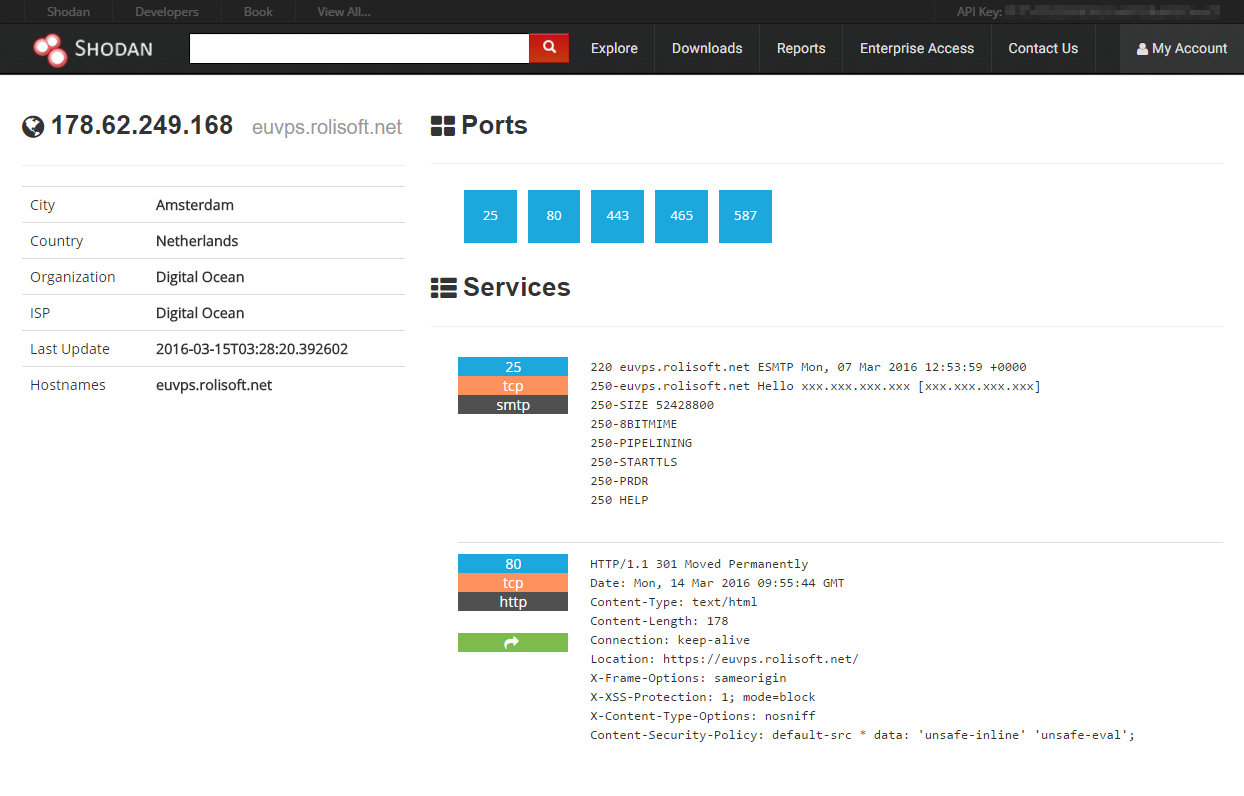
\includegraphics[scale=0.355]{shodan.png}
		\caption{Shodan report on 178.62.249.168}
		\label{shodanscr}
	\end{figure}
	
	In order to use Shodan data in the application developed within the scope of this thesis, the user has to create a free account at \url{https://shodan.io/} and specify the generated API key to the application via the \mintinline{bash}{--shodan-key} argument.
	
	Implementation-wise, the \mintinline{cpp}{ShodanScanner} component takes care of contacting the Shodan JSON API interface and retrieving the data available for the specified IP addresses. This component extends the \mintinline{cpp}{HostScanner} class, and as such it is possible to substitute the default scanner to Shodan data for any scanning needs.

\subsubsection{Censys} \label{ssec:censys}
\subsubsectionhu{Censys} \subsubsectionro{Censys}

	Censys\cite{censys15} is a project created and run by the Regents of the University of Michigan. Similarly to the previously discussed service, it also gathers its data by regular Internet-wide scanning efforts. It allows developers and security researchers to initiate structured queries, full-text search queries or raw SQL queries from their web interface or the exposed RESTful API. Figure \ref{censysscr} shows the data readily available on the service for a queried IP address.
	
	\begin{figure}[!htbp]
		\centering
		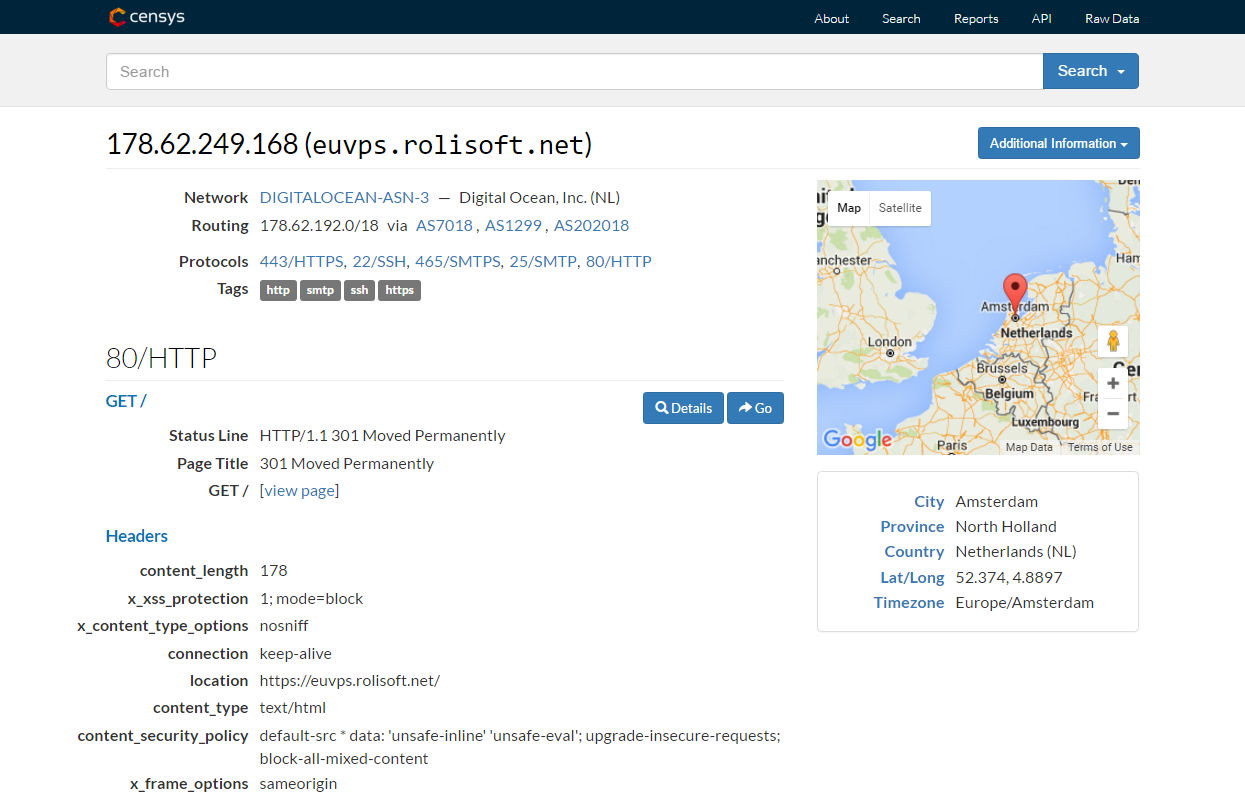
\includegraphics[scale=0.355]{censys.png}
		\caption{Censys report on 178.62.249.168}
		\label{censysscr}
	\end{figure}
	
	The network scanner in use by the service, namely ZMap\cite{zmap13}, and its various components are open-source. The raw data generated by this scanner during an Internet-wide scan is also available for download at the Censys website for anyone to freely consume.
	
	In order to use Censys data in the application developed within the scope of this thesis, the user has to create a free account at \url{https://censys.io/} and specify the generated UID and secret key to the application via the \mintinline{bash}{--censys-key} argument.
		
	Implementation-wise, the \mintinline{cpp}{CensysScanner} component takes care of contacting the Censys JSON API interface and retrieving the data available for the specified IP addresses. Similarly, this component also extends the \mintinline{cpp}{HostScanner} class, and as such it is possible to substitute the default scanner to Censys data for any scanning needs.

\subsubsection{Amalgamation}
\subsubsectionhu{Egyesítés} \subsubsectionro{Amalgamare}

	The \mintinline{cpp}{PassiveScanner} component of the application initiates the requested scan tasks on both Shodan[\ref{ssec:shodan}] and Censys[\ref{ssec:censys}], merging the results at the end.
	
	During the development phase of the application it was found that generally both services have had data on a requested IP address, but most of the times one of the services discovered more ports, have done much deeper analysis, or the information is more useful than at the competitor service.
	
	One concrete example would be where one service was somehow identified and banned from indexing an IP address, as shown in listing \ref{shodanban}, yet the other one was able to freely access it and has data available as a result, as shown in listing \ref{censysnoban}.
	
	\begin{listing}[H]
		\begin{minted}[style=pastie]{http}
			HTTP/1.1 403 You are banned from this site.  Please contact via a different client configuration if you believe that this is a mistake.
			Content-Type: text/html; charset=utf-8
			Date: Wed, 16 Mar 2016 01:17:18 GMT
			Retry-After: 5
			Server: Varnish
			X-Varnish: 2115087
			Content-Length: 590
			Connection: keep-alive
		\end{minted}
		\caption{Example response of 54.193.103.xyz for Shodan with a ban message}
		\label{shodanban}
	\end{listing}
		
	\begin{listing}[H]
		\begin{minted}[style=pastie]{http}
			HTTP/1.1 200 OK
			Content-Length: 3770
			Vary: Accept-Encoding
			Server: nginx/1.8.0
			Connection: keep-alive
			Last-Modified: Fri, 28 Aug 2015 19:43:39 GMT
			Content-Type: text/html
			Accept-Ranges: bytes
		\end{minted}
		\vspace{-5pt}
		\begin{minted}[style=borland,firstnumber=9]{html}
			 
			<!DOCTYPE html PUBLIC "-//W3C//DTD XHTML 1.1//EN" "http://www.w3.org/TR/xhtml11/DTD/xhtml11.dtd">
			<html xmlns="http://www.w3.org/1999/xhtml" xml:lang="en">
			<head>
			<!-- rest of the page omitted -->
		\end{minted}
		\caption{Example response of 54.193.103.xyz for Censys without a ban message}
		\label{censysnoban}
	\end{listing}

	It should be also noted that the underlying server software is not exposed to the banned party in listing \ref{shodanban}, but the non-banned party in listing \ref{censysnoban} has their request forwarded from the load-balancer to the backend, revealing itself to be ``nginx 1.8.0,'' a version with at least one \textbf{known remotely-exploitable vulnerability}\cite{nginxcve} at this time.

	In cases where both services return a service banner for a specific port, the longer banner is chosen during the amalgamation phase. One of the reasons for this decision was because ban messages are generally shorter\cite{qualys11} in order to avoid denial of service attacks. The other reason was because a longer banner generally means that the service in question possibly probed the port further (e.g. `STARTTLS' command sent to SMTP servers by Censys, but not by Shodan) which allows the pattern matching component described in \ref{ssec:patternmatch} to have more data available.

\subsection{External Reconnaissance} \label{ssec:nmapscan}
\subsectionhu{Külső Feltérképezés} \subsectionro{Scanare Externală}

	This section presents the \mintinline{cpp}{NmapScanner} component of the application which executes an external application in order to scan the requested ports, and then parses the results of the $3^{rd}$-party application for further processing within the $1^{st}$-party application.
	
	While the application implements a wide range of protocol scanners as discussed in sections \ref{ssec:icmpping} through \ref{ssec:udpscan}, with an unified interface for task parallelization as discussed in section \ref{ssec:tasks}, as a measure of redundancy, the users are given the choice of using an external scanner for their reconnaissance purposes.
	
	The component, as its name suggests, supports \textit{nmap} out-of-the-box as an alternative scanner, however any $3^{rd}$-party application which generates nmap-compatible XML-based reports can be used. One such example is the \textit{masscan} scanner.
	
	In order to use nmap for scanning, the \mintinline{batch}{nmap} executable has to be accessible from within the \mintinline{batch} environmental variable.

\newpage
\subsection{Class Hierarchy of Data Reconnaissance Components}
\subsectionhu{Adatszerző Komponensek Osztályhierarhiája} \subsectionro{Ierarhia de Clasă a Componentelor Colectoare de Date}

	\begingroup
	\hypersetup{linkcolor=blue}
	\begin{figure}[!htbp]
		\centering
		\begin{tikzpicture}[scale=0.85,transform shape]
			\node at (0,0) {HostScanner};
			\draw  (-1.5,0.5) rectangle (1.5,-0.5);
			\node at (-2,-3) {InternalScanner};
			\node at (-6,-3) {ArpPinger$^{\ref{ssec:arpping}}$};
			\node at (2,-3) {NmapScanner$^{\ref{ssec:nmapscan}}$};
			\draw  (-3.75,-2.5) rectangle (-0.25,-3.5);
			\draw  (0.25,-2.5) rectangle (3.75,-3.5);
			\draw  (-7.5,-2.5) rectangle (-4.5,-3.5);
			\node (v3) at (-6,-2.5) {};
			\node (v1) at (0,-0.5) {};
			\node (v2) at (-2,-2.5) {};
			\node (v4) at (2,-2.5) {};
			\draw [es] (v1) edge (v2);
			\draw [es] (v1) edge (v3);
			\draw [es] (v1) edge (v4);
			\node at (6,-3) {PassiveScanner};
			\draw  (4.5,-2.5) rectangle (7.5,-3.5);
			\node (v3_1) at (6,-2.5) {};
			\draw [es] (v1) edge (v3_1);
			\node at (3.5,-6) {ShodanScanner$^{\ref{ssec:shodan}}$};
			\draw  (1.5,-5.5) rectangle (5.5,-6.5);
			\node (v3_2) at (3.5,-5.5) {};
			\node at (8.5,-6) {CensysScanner$^{\ref{ssec:censys}}$};
			\draw  (6.5,-5.5) rectangle (10.5,-6.5);
			\node (v3_3) at (8.5,-5.5) {};
			\node (v5) at (6,-3.5) {};
			\draw [triangle 60-triangle 60] (v5) edge (v3_2);
			\draw [triangle 60-triangle 60] (v5) edge (v3_3);
			\node at (-2,-6) {ServiceScanner};
			\draw  (-3.75,-5.5) rectangle (-0.25,-6.5);
			\node at (-2,-9) {TcpScanner$^{\ref{ssec:tcpscan}}$};
			\node at (-6.25,-9) {IcmpScanner$^{\ref{ssec:icmpping}}$};
			\node at (2,-9) {UdpScanner$^{\ref{ssec:udpscan}}$};
			\draw  (-3.75,-8.5) rectangle (-0.25,-9.5);
			\draw  (0.25,-8.5) rectangle (3.75,-9.5);
			\draw  (-8,-8.5) rectangle (-4.5,-9.5);
			\node (v3_4) at (-6.25,-8.5) {};
			\node (v1_1) at (-2,-6.5) {};
			\node (v2_1) at (-2,-8.5) {};
			\node (v4_1) at (2,-8.5) {};
			\node (v6) at (-2,-3.5) {};
			\node (v7) at (-2,-5.5) {};
			\draw [dashed,-diamond]  (v6) edge (v7);
			\draw [es] (v1_1) edge (v2_1);
			\draw [es] (v1_1) edge (v3_4);
			\draw [es] (v1_1) edge (v4_1);
		\end{tikzpicture}
		\caption{Class Hierarchy of Data Reconnaissance Components}
		\label{classhierdata}
	\end{figure}
	\endgroup

\subsection{Multiplexing Task Runner} \label{ssec:tasks}
\subsectionhu{Feladatok Párhuzamosítása} \subsectionro{Paralelizarea Sarcinilor}
	
	A ``task'' in this context is defined to be the action of scanning a port on an IP address for a specified protocol. Such tasks mostly consist of sending IP packets back and forth followed by waiting for their acknowledgment or lack thereof.
	
	As such, the parallelization method of using a thread pool and multiple threads is not efficient, since most threads would spend their time sleeping. Given the costly nature of thread spawning and managing, this is not efficient unless more lightweight threads can be spawned, such as `goroutines' in the Go programming language.
	
	The application instead implements a consumer-producer queue for storing and retrieving its tasks during scheduling, as shown in figure \ref{taskqueue}.
	
	\begin{figure}[!htbp]
		\centering
		\begin{tikzpicture}
			\draw[color=gray,fill=gray] (0,-0.5) rectangle (-0.5,0);
			\draw[color=gray,fill=gray] (-1,-0.5) rectangle (-1.5,0);
			\draw[color=gray,fill=gray] (-2,-0.5) rectangle (-2.5,0);
			\draw[color=gray,fill=gray] (-3,-0.5) rectangle (-3.5,0);
			\draw[color=gray,fill=gray] (-4,-0.5) rectangle (-4.5,0);
			\draw (-5,0.25) -- (0.5,0.25);
			\draw (-5,-0.75) -- (0.5,-0.75);
			\node at (-2.25,0.75) {Queue of Tasks};
			\node (v1) at (0.5,-0.25) {};
			\draw [es](v1) -- (1.5,-0.25);
			\node at (-3.75,1.75) {Task Producer};
			\node at (-0.85,-2) {Enqueue due to I/O Wait};
			\node at (2.25,-0.25) {\huge \faCogs};
			\node at (2.25,-1.15) {Run Task};
			\node at (-5.6,1.75) {\huge \faPlusCircle};
			\node at (-3.75,-2) {\huge \faHourglassHalf};
			\node (v5) at (3,-0.25) {};
			\draw [es](v5) -- (4,0.75);
			\draw [es] plot[smooth, tension=.7] coordinates {(-4.5,-2) (-5.1,-1.55) (-5.3,-0.85) (-5.15,-0.35)};
			\draw [es] plot[smooth, tension=.7] coordinates {(-4.75,1.25) (-5.2,0.95) (-5.35,0.4) (-5.15,-0.15)};
			\node at (2,1.25) {\huge \faCheck};
			\node at (4.25,1.25) {Finished with Task};
			\draw [es] plot[smooth, tension=.7] coordinates {(3.15,-0.4) (3.55,-1.2) (3.1,-1.8) (1.75,-2)};
		\end{tikzpicture}
		\caption{Consumer-Producer Queue Process for Tasks}
		\label{taskqueue}
	\end{figure}
	
	\begin{figure}[!htbp]
		\centering
		\begin{tikzpicture}
			\node at (-4.5,1.5) {Send initial payload};
			\node at (0,1.5) {Check for reply};
			\node at (4,1.5) {Read reply};
			\node at (8.25,1.5) {Finish};
			\draw [es](-2.5,1.5) -- (-1.5,1.5);
			\draw [es](1.5,1.5) -- (2.75,1.5);
			\draw [es] plot[smooth, tension=.7] coordinates {(4,2) (3.25,2.5) (0.75,2.5) (0,2)};
			\draw [es](5.25,1.5) -- (7.25,1.5);
			\node at (2,3) {\textit{if no reply}};
			\node[align=center] at (6.25,2.25) {\textit{if wait expired}\\\textit{or got reply}};
			\node at (-4.5,0.25) {\textit{Phase 1}};
			\node at (1.75,0.25) {\textit{Phase 2}};
			\node at (8.25,0.25) {\textit{Phase 3}};
			\draw (-6,0.75) -- (-3,0.75);
			\draw (-1.25,0.75) -- (4.75,0.75);
			\draw (7.5,0.75) -- (9,0.75);
			\draw[color=gray] (-2.75,0.75) -- (-1.5,0.75);
			\draw[color=gray] (5,0.75) -- (7.25,0.75);
			\node[color=gray] at (-2.1,0.25) {I/O Wait};
			\node[color=gray] at (6.2,0.25) {I/O Wait};
		\end{tikzpicture}
		\caption{Phases of an UDP scan as implemented by component in section \ref{ssec:udpscan}}
		\label{taskudp}
	\end{figure}
	
	In figure \ref{taskudp}, the phases of an UDP scan task are shown. Each `phase' shows up in the queue as a different `task.' As a result of this scheduling and task multiplexing, one thread can handle all the scanning tasks needs.
	
	All tasks are implemented to use their sockets in a non-blocking mode, as such, as soon as one task has sent an IP packet and is about to wait for the results of its I/O operation, it instead goes into the back of the queue.
	
	Once the whole queue has been looped to collect the results of the previously initiated I/O operations, the aforementioned task will have a chance to collect its own operation results.
	
	The multiplexing task runner uses a lock-free thread-safe underlying queue container, namely the concurrent FIFO implementation in Boost, \mintinline{cpp}{boost::lockfree::queue<T>}. As a result, for heavy workloads when excessive resources are available, the task runner can theoretically use multiple consumers on the same queue.
	
\subsection{Protocol Tokenization} \label{ssec:tokenizer}
\subsectionhu{Protokoll Értelmezés} \subsectionro{Interpretor de Protocoale}
	
	In order to improve the quality of the input for the CPE matcher component (further discussed in \ref{ssec:matchcpe}) and thereby minimizing the chances of false positives, the application makes a best effort to try recognizing and tokenizing the extracted service banners.
	
	The server replies are not fully parsed using a protocol-aware parser, instead it aims to either \textit{a)} extract server names, versions and operating system tags, or if that is not possible, \textit{b)} clean any known protocol strings, leaving only implementation-specific strings in the service banner.
	
	Currently there are two protocol tokenizers implemented, and these are run in order of protocol popularity when a service banner needs to be cleaned. An API is exposed which does this, \mintinline{cpp}{ProtocolTokenizer::AutoTokenize(const std::string& banner)}.
	
\subsubsection{Hyper-Text Transfer Protocol Tokenizer}
\subsubsectionhu{HTTP Értelmező} \subsubsectionro{Interpretor HTTP}
	
	The first tokenizer is \mintinline{cpp}{HttpTokenizer}, which decides whether the specified service banner contains a valid HTTP header, and if so, proceeds to tokenize it. During tokenization, it will try to extract product names and version numbers from the appropriate places.
	
	The HTTP protocol has the `Server' and `X-Powered-By' header fields, which are generally used by software to indicate their name and version number. Unfortunately, the exact listing methodology is not standardized, as such different software may use different separators and notation to indicate their existence, version number, any vendor patches and possibly the operating system. Since these fields may have multiple products listed, the tokenizer makes sure to extract all the product names including any associated version numbers into separate tokens.
	
	\begin{listing}[H]
		\begin{minted}[style=pastie]{http}
			HTTP/1.1 200 OK
			Server: nginx/1.9.12 (Ubuntu)
			X-Powered-By: PHP/5.6.19
			Date: Fri, 11 Mar 2016 16:04:07 GMT
			Connection: close
		\end{minted}
		\caption{Example HTTP service banner}
		\label{httpsvcbnr}
	\end{listing}
	
	The HTTP service banner shown in listing \ref{httpsvcbnr} is produced by nginx 1.9.12 with PHP 5.6.19 installed on an Ubuntu distribution. When processed by the implemented tokenizer, it will produce the elements shown in listing \ref{httpsvcbnrtokens}.
	
	\begin{listing}[H]
		\begin{minted}[style=perldoc]{js}
			[
				// token,           later mapped to,           by component
				"nginx/1.9.12",  // cpe:/a:nginx:nginx:1.9.12, CpeDictionaryMatcher
				"Ubuntu",        // cpe:/o:canonical:ubuntu,   OpSysMatcher
				"PHP/5.6.19"     // cpe:/a:php:php:5.6.19,     CpeDictionaryMatcher
			]
		\end{minted}
		\caption{Extracted tokens from banner in listing \ref{httpsvcbnr}}
		\label{httpsvcbnrtokens}
	\end{listing}
	
	However, if the service banner being analyzed does not contain a valid HTTP header, the next tokenizer in order of protocol popularity to be tried is the \mintinline{cpp}{ThreeDigitTokenizer}, hereinafter referred to as the ``SMTP tokenizer'' for simplicity's sake.

\subsubsection{Generic Fallback Tokenizer}
\subsubsectionhu{Generikus Értelmező} \subsubsectionro{Interpretor Generic}
	
	The ``three-digit'' tokenizer is a general purpose solution for parsing protocols which use a three-digit response in their protocol to indicate message type/category of a given server reply. Such protocols include SMTP, NNTP, FTP and a few more. For these protocols, however, unfortunately there is no standardized way to announce server name and version (like the `Server' header in the HTTP protocol) and as such the server name is generally casually announced in the informational level welcome message part of the service banner. The informational messages are generally within the range of $200-299$, however this might vary depending on the actual protocol.
	
	\begin{listing}[H]
		\begin{minted}{matlab}
			220 example.com ESMTP Exim 4.87 #2 Fri, 11 Mar 2016 16:05:06 +0000
		\end{minted}
		\caption{Example SMTP service banner}
		\label{smtpsvcbnr}
	\end{listing}
		
	The SMTP service banner shown in listing \ref{smtpsvcbnr} is produced by Exim 4.87 listening on port 25. This banner is sent as a `greeting' as soon as the client connects to the server. This is favorable, since no further protocol probes are required to be sent in order to get a processable service banner. When this banner is processed by the implemented tokenizer, it will produce the elements shown in listing \ref{smtpsvcbnrtokens}.
		
	\begin{listing}[H]
		\begin{minted}[style=perldoc]{js}
			[
				// token,                later mapped to,       by component
				"ESMTP Exim 4.87 #2", // cpe:/a:exim:exim:4.87, CpeDictionaryMatcher
			]
		\end{minted}
		\caption{Extracted tokens from banner in listing \ref{smtpsvcbnr}}
		\label{smtpsvcbnrtokens}
	\end{listing}
	
	It should be noted that the ``perfect'' token would be \mintinline{matlab}{Exim 4.87}, however as previously mentioned, the server name and version are not clearly advertised. As such, the processing of the banner starts by removing the protocol-specific strings, namely the response code (\mintinline{matlab}{220}), the host name (\mintinline{py}{example.com}), and the date (\mintinline{matlab}{Fri, 11 Mar 2016 16:05:06 +0000}). This leaves us with the implementation-specific string of \mintinline{matlab}{ESMTP Exim 4.87 #2}.
	
	The tokenizer implementation will try to remove as much non-implementation-specific tokens as possible, however in cases where a specific element cannot be determined with a high degree of certainty whether it is a protocol or implementation-specific string, the tokenizer will instead leave it in. This decision was made in order to ensure that the tokenizer does not remove any elements which are required for the CPE matcher during entry matching. If an element is left in falsely, it does not affect the scoring of the CPE matcher, however, if it was falsely removed, it could completely prevent the matching of that entry.
	
	If all of the implemented tokenizers fail to process a service banner, it will be sent to the next stage of discovery (usually to component described in \ref{ssec:matchcpe}) as one token, containing the whole service banner.
	
\subsection{Pattern Matching of Service Banners} \label{ssec:patternmatch}
\subsectionhu{Szerverek Minta-alapú Beazonosítása} \subsectionro{Identificare Software pe Bază de Model}

	The purpose of the \mintinline{cpp}{ServiceRegexMatcher} component of the application is to take the original full service banner (without any tokenization) as an input, and match it against a database of regular expressions, which in turn are mapped to their own CPE names.

	\begin{listing}[H]
		\begin{minted}{matlab}
			^HTTP/1\.[01] \d{3}.*\r\nServer: nginx(?:/([\d.]+))?
		\end{minted}
		\caption{Example regular expression to match \mintinline{matlab}{cpe:/a:nginx:nginx}}
		\label{nginxregex}
	\end{listing}
	
	The example regular expression in listing \ref{nginxregex} matches against the response headers produced by the HTTP server software ``nginx''. See the service banner in listing \ref{httpsvcbnr} for an example that would be matched. Furthermore, the listed regular expression contains an optional capture group, which captures the version number. If the version number is listed in the service banner, the matcher component would return the CPE name \mintinline{matlab}{cpe:/a:nginx:nginx:1.9.12}, while without a version number listed, it will still return the CPE name \mintinline{matlab}{cpe:/a:nginx:nginx}.
	
	This behavior is different from the matcher described in section \ref{ssec:matchcpe}: whereas here a CPE name can be produced with high confidence with or without a known version number, the CPE dictionary-based matcher \textit{requires} a known version number, since it plays a pivotal role in the identifying and scoring process.
	
\subsubsection{Inferring Products Without Express Announcement}
\subsubsectionhu{Identitás Kikövetkeztetése Névhírdetés Nélkül} \subsubsectionro{Deducerea Identității fără Anunțul cu Nume}
	
	While the example presented in listing \ref{nginxregex} is rather straight-forward, the pattern matcher method can be used in a more subtle way, for example to match software which are not advertising their name or version number.
	
	\begin{listing}[H]
		\begin{minted}{matlab}
			^554 SMTP synchronization error\r\n
		\end{minted}
		\caption{Example regular expression to match \mintinline{matlab}{cpe:/a:exim:exim}}
		\label{eximregex}
	\end{listing}
	
	The example presented in listing \ref{eximregex} is a regular expression which matches an error message produced by the SMTP server software ``exim''. The reason why it is possible to determine this fact with a high confidence, is because exim is the only software returning this exact error message verbatim. Other SMTP servers will have a similar error message for this problem, with the same error code, but not with this same exact error message, as the messages themselves are not standardized byte-by-byte.
	
	\begin{multicols}{2}
		\begin{listing}[H]
			\begin{minted}{matlab}
				220 example-1.com ESMTP Sat, 12 Mar 2016 17:14:06 +0000
				EHLO client-1.com
				250-example-1.com Hello client-1.com [2a02:2f07:d18d:1100::cake]
				250-SIZE 52428800
				250-8BITMIME
				250-PIPELINING
				250-STARTTLS
				250-PRDR
				250 HELP
			\end{minted}
			\caption{Exim $\ge 4.83$}
			\label{eximwiprdr}
		\end{listing}
		\begin{listing}[H]
			\begin{minted}{matlab}
				220 example-2.com ESMTP Sat, 12 Mar 2016 16:12:25 +0000
				EHLO client-2.com
				250-example-2.com Hello client-2.com [2a02:2f07:d18d:1100::cake]
				250-SIZE 20971520
				250-8BITMIME
				250-PIPELINING
				250-AUTH PLAIN LOGIN
				250-STARTTLS
				250 HELP
			\end{minted}
			\caption{Exim $< 4.83$}
			\label{eximwoprdr}
		\end{listing}
	\end{multicols}
	
	It is even possible to associate a version number to the software behind the port. For example, exim has implemented ``SMTP Service Extension for Per-Recipient Data Responses'' in version 4.83, and it advertises this capability as `PRDR' after the handshake, as seen in listing \ref{eximwiprdr} versus the handshake of an older version in listing \ref{eximwoprdr}.
	
	A regular expression can be written to inspect the advertised capability list, and make an educated guess stating that the version of the software is 4.83 or older. This can be further improved by creating a pattern which matches a change which only applies to versions 4.86 and older, at which point it can deduced that the inspected service banner was produced by exim between the versions of $4.83-4.86$.
	
	For open-source software, it is possible to compare the source between different releases and check which publicly visible string changed, in order to write a pattern for detecting that range of versions. Building such a database of patterns, however, is beyond the scope of this project, and would be more suited for a community-sourced project.
	
\subsection{Matching of CPE Tokens in Service Banners} \label{ssec:matchcpe}
\subsectionhu{Szerverek CPE-alapú Beazonosítása} \subsectionro{Identificare Software pe Bază de CPE}

	As discussed in \ref{ssec:vulndbs}, the \textit{National Institute of Standards and Technology} runs a \textit{National Vulnerability Database}. The \mintinline{cpp}{CpeDictionaryMatcher} component presented within this section makes use of the publicly distributed, freely available and daily updated \textit{Common Platform Enumeration Dictionary}.
	
	The \textit{CPE} is a naming scheme for hardware, software and operating systems\cite{cpe22}. Its v2.2 format is \mintinline{matlab}{cpe:/type:vendor:product:version:update:edition:language} where the `type' component can be \mintinline{matlab}{h} for `hardware', \mintinline{matlab}{o} for `operating system' and \mintinline{matlab}{a} for `application', while the rest of the components are self-explanatory.
	
	For example, the CPE name for ``nginx 1.3.9'' is \mintinline{matlab}{cpe:/a:igor_sysoev:nginx:1.3.9}.
	
	The aforementioned \textit{CPE dictionary} is a list of CPE names aggregated and maintained by NIST which are known to be vulnerable, i.e. have associated entries in the \textit{CVE database}.
	
	In listing \ref{nginxcpe} an excerpt is shown, presenting an entry from the dictionary for the ``nginx 1.9.9'' software.
	
	\begin{listing}[H]
		\begin{minted}[style=borland]{xml}
			<cpe-item name="cpe:/a:nginx:nginx:1.9.9">
				<title xml:lang="en-US">Nginx 1.9.9</title>
				<references>
					<reference href="http://nginx.org/">Product</reference>
					<reference href="http://nginx.org/en/CHANGES">Change Log</reference>
				</references>
				<cpe-23:cpe23-item name="cpe:2.3:a:nginx:nginx:1.9.9:*:*:*:*:*:*:*"/>
			</cpe-item>
		\end{minted}
		\caption{CPE entry for nginx 1.9.9}
		\label{nginxcpe}
	\end{listing}
	
	Unfortunately, the CPE names are not advertised in the service banners, nor is there a direct standard to map CPE names to service banners, or any other straight-forward solution on mapping them. In paper \cite{shovat15}, the authors have tackled with the same issue of processing and mapping the entries to service banners. The method presented within the paper was the basis for the implementation of the CPE matcher component in the application developed within the scope of this thesis.
	
\subsubsection{Implementation Overview}
\subsubsectionhu{Kivitelezés Áttekintése} \subsubsectionro{Prezentare Generală}
	
	The current implementation of the CPE matcher component loads a preprocessed version of the CPE dictionary into its memory, where the CPE names are tokenized and irrelevant data (such as product links) are stripped for memory efficiency. Listing \ref{ciscotokens} presents the tokens loaded into memory for an example CPE name. For the exact implementation, see the structures within the header file of the \mintinline{cpp}{CpeDictionaryMatcher} class.
	
	\begin{listing}[H]
		\begin{minted}[style=perldoc]{js}
			CpeEntry {
				// cpe:/o:cisco:ios
				"ProductSpecificTokens": ["cisco", "ios"],
				"Versions": [
					CpeVersionEntry {
						// cpe:/o:cisco:ios:12.2sxi
						"VersionNumber": "12.2",
						"VersionSpecificTokens": ["sxi"]
					},
					CpeVersionEntry {
						// cpe:/o:cisco:ios:12.2sxh
						"VersionNumber": "12.2",
						"VersionSpecificTokens": ["sxh"]
					}
					// [further versions omitted]
				]
			}
		\end{minted}
		\caption{Approximate internal representation of tokens for \mintinline{matlab}{cpe:/o:cisco:ios:12.2sxi}}
		\label{ciscotokens}
	\end{listing}
	
	During the tokenization process, the `vendor' and `product' components of the CPE name are matched against the regular expression \mintinline{matlab}{([a-z][a-z0-9]+)} in order to extract all words individually, ignoring one character words and those starting with a number.
	
	Doing so, the resulting array will end up looking like \mintinline[style=vs]{js}{["apache", "tomcat"]} for the example CPE name \mintinline{matlab}{cpe:/a:apache:tomcat:4.1.36}.
	
	The version component of the CPE contains in some cases irrelevant characters or non-standard version notation. In order to work around this, the version number is extracted from the component using the regular expression \mintinline{matlab}{\d+\.(?:\d+\.)*\d+}, which requires at least two numbers separated by a dot.
	
	If the version number contains any words, these are extracted with the aforementioned regular expression in the tokenization phase. As such, in the case of the CPE name \mintinline{matlab}{cpe:/o:cisco:ios:12.2sxi}, there will be an array of `version-specific tokens' consisting of the word \mintinline[style=vs]{js}{["sxi"]}.
	
	During CPE matching the entries are iterated, checking to see if the product-specific tokens match. If all of the tokens match, the entry-specific versions are iterated, checking to see if any of the version numbers are present in the input. If so, version-specific tokens are checked as well. A version is not considered a match if the version number matches, but even just one of the version-specific tokens do not.
	
	There are entries where multiple versions may match within the same product, such edge cases are discussed in subsection \ref{ssec:cpeedges}. In situations like these, a single version number is selected as the winner, which is determined by the distance of the tokens to the version number. The further a token is from the version number, the lesser it is considered to be relevant.
	
	For product names however, if multiple products (including their complete version numbers with tokens) match, all of the matches will be returned. The reason for this decision is because a service banner may name multiple software in use, but not multiple versions of the same software to be in use. In listing \ref{httpsvcbnr}, the service banner reveals the existence of three products, namely ``nginx 1.9.12,'' ``PHP 5.6.19'' and ``Ubuntu.''
	
\subsubsection{Handling of Edge Cases} \label{ssec:cpeedges}
\subsubsectionhu{Élesetek Kezelése} \subsubsectionro{Soluționarea Cazurilor de Margine}

	The now-defunct \textit{Sun Microsystems} vendor identifier is ``sun'', resulting in CPE names such as \mintinline{matlab}{cpe:/a:sun:jre}, \mintinline{matlab}{cpe:/a:sun:jdk} and \mintinline{matlab}{cpe:/o:sun:solaris:10.0}. The problematic part with this token is that most protocols, such as SMTP and HTTP, return the current date in the RFC 1123 format\cite{rfc2616}, which looks like this: ``Sun, 14 Mar 2016 16:33:02 GMT''.
	
	The first component of the date is the shortened three-letter English name of the day, which on Sundays is ``Sun''. This introduces a `random' element into the equation, as the scoring system of the CPE matcher would rank CPEs from the \textit{Sun Microsystems} vendor higher, as the ``sun'' token is now present in the service banner.
	
	\begin{listing}[H]
		\begin{minted}{matlab}
			Cisco IOS Software, s72033_rp Software (s72033_rp-IPSERVICESK9_WAN-M), Version 12.2(33)SXI3, RELEASE SOFTWARE (fc2)
			Technical Support: http://www.cisco.com/techsupport
			Copyright (c) 1986-2009 by Cisco Systems, Inc.
			Compiled Tue 27-Oct-09 11:12 by prod_
		\end{minted}
		\caption{Example telnet service banner of Cisco routers}
		\label{ciscosvcbnr}
	\end{listing}

	Another example would be Cisco's version numbering and their telnet service banners. In listing \ref{ciscosvcbnr}, the service banner of \mintinline{matlab}{cpe:/o:cisco:ios:12.2sxi3} is shown. The problematic part arises from the fact that Cisco has the same version number $12.2$ with the patch level specified as ``by'': \mintinline{matlab}{cpe:/o:cisco:ios:12.2by}.
	
	If one were to tokenize the two CPE names, they would get two arrays which would look like these: \mintinline[style=vs]{js}{["cisco", "ios", "sxi"]} and \mintinline[style=vs]{js}{["cisco", "ios", "by"]}. The version number and the first two tokens from both arrays would match, however so would both ``sxi'' and ``by''. On lines 3 and 4 of \ref{ciscosvcbnr} the copyright and compilation notices both contain the word/token ``by''.

	The aforementioned ShoVAT\cite{shovat15} paper solved this issue by weighing tokens around the version number more than those further from the version number, which solution is ultimately what the application written within the scope of this thesis has also settled with on one hand.
	
	However, a different solution was also implemented to combat this. The protocol tokenizer component discussed in \ref{ssec:tokenizer} was developed for the express purpose of extracting product names and versions from a service banner, or if that is not possible, then removing irrelevant parts, such as dates and non-informational messages.
		
	\begin{listing}[H]
		\begin{minted}[style=borland]{xml}
			<entry id="CVE-2016-0742">
				<summary>The resolver in nginx before 1.8.1 and 1.9.x before 1.9.10 allows remote attackers to cause a denial of service (invalid pointer dereference and worker process crash) via a crafted UDP DNS response.</summary>
				<vulnerable-software-list>
					<product>cpe:/a:nginx:nginx:1.9.9</product>
					<product>cpe:/a:nginx:nginx:1.9.8</product>
					<product>cpe:/a:nginx:nginx:1.9.7</product>
					<product>cpe:/a:nginx:nginx:1.9.6</product>
					<!-- [several other versions omitted] -->
				</vulnerable-software-list>
				<cvss>
					<base_metrics>
						<score>5.0</score>
						<access-vector>NETWORK</access-vector>
						<access-complexity>LOW</access-complexity>
						<authentication>NONE</authentication>
						<confidentiality-impact>NONE</confidentiality-impact>
						<integrity-impact>NONE</integrity-impact>
						<availability-impact>PARTIAL</availability-impact>
						<source>http://nvd.nist.gov</source>
					</base_metrics>
				</cvss>
				<references xml:lang="en" reference_type="UNKNOWN">
					<source>CONFIRM</source>
					<reference href="https://bugzilla.redhat.com/show_bug.cgi?id=1302587" xml:lang="en">Bug 1302587</reference>
				</references>
				<references xml:lang="en" reference_type="UNKNOWN">
					<source>DEBIAN</source>
					<reference href="http://www.debian.org/security/2016/dsa-3473" xml:lang="en">DSA-3473</reference>
				</references>
				<!-- [several other references omitted] -->
				<published-datetime>2016-02-15T14:59:00.107-05:00</published-datetime>
				<last-modified-datetime>2016-02-29T18:40:11.667-05:00</last-modified-datetime>
			</entry>
		\end{minted}
		\caption{CVE-2016-0742 entry affecting nginx 1.9.9}
		\label{nginxcve}
	\end{listing}

\newpage
\section{Bibliography}
\sectionhu{Bibliográfia} \sectionro{Bibliografie}

	\begingroup
	\renewcommand{\section}[2]{}
	\renewcommand{\markboth}[2]{}
		\bibliography{thesis}
		\bibliographystyle{thesis}
	\endgroup

\end{document}